\documentclass[1p]{elsarticle_modified}
%\bibliographystyle{elsarticle-num}

%\usepackage[colorlinks]{hyperref}
%\usepackage{abbrmath_seonhwa} %\Abb, \Ascr, \Acal ,\Abf, \Afrak
\usepackage{amsfonts}
\usepackage{amssymb}
\usepackage{amsmath}
\usepackage{amsthm}
\usepackage{scalefnt}
\usepackage{amsbsy}
\usepackage{kotex}
\usepackage{caption}
\usepackage{subfig}
\usepackage{color}
\usepackage{graphicx}
\usepackage{xcolor} %% white, black, red, green, blue, cyan, magenta, yellow
\usepackage{float}
\usepackage{setspace}
\usepackage{hyperref}

\usepackage{tikz}
\usetikzlibrary{arrows}

\usepackage{multirow}
\usepackage{array} % fixed length table
\usepackage{hhline}

%%%%%%%%%%%%%%%%%%%%%
\makeatletter
\renewcommand*\env@matrix[1][\arraystretch]{%
	\edef\arraystretch{#1}%
	\hskip -\arraycolsep
	\let\@ifnextchar\new@ifnextchar
	\array{*\c@MaxMatrixCols c}}
\makeatother %https://tex.stackexchange.com/questions/14071/how-can-i-increase-the-line-spacing-in-a-matrix
%%%%%%%%%%%%%%%

\usepackage[normalem]{ulem}

\newcommand{\msout}[1]{\ifmmode\text{\sout{\ensuremath{#1}}}\else\sout{#1}\fi}
%SOURCE: \msout is \stkout macro in https://tex.stackexchange.com/questions/20609/strikeout-in-math-mode

\newcommand{\cancel}[1]{
	\ifmmode
	{\color{red}\msout{#1}}
	\else
	{\color{red}\sout{#1}}
	\fi
}

\newcommand{\add}[1]{
	{\color{blue}\uwave{#1}}
}

\newcommand{\replace}[2]{
	\ifmmode
	{\color{red}\msout{#1}}{\color{blue}\uwave{#2}}
	\else
	{\color{red}\sout{#1}}{\color{blue}\uwave{#2}}
	\fi
}

\newcommand{\Sol}{\mathcal{S}} %segment
\newcommand{\D}{D} %diagram
\newcommand{\A}{\mathcal{A}} %arc


%%%%%%%%%%%%%%%%%%%%%%%%%%%%%5 test

\def\sl{\operatorname{\textup{SL}}(2,\Cbb)}
\def\psl{\operatorname{\textup{PSL}}(2,\Cbb)}
\def\quan{\mkern 1mu \triangleright \mkern 1mu}

\theoremstyle{definition}
\newtheorem{thm}{Theorem}[section]
\newtheorem{prop}[thm]{Proposition}
\newtheorem{lem}[thm]{Lemma}
\newtheorem{ques}[thm]{Question}
\newtheorem{cor}[thm]{Corollary}
\newtheorem{defn}[thm]{Definition}
\newtheorem{exam}[thm]{Example}
\newtheorem{rmk}[thm]{Remark}
\newtheorem{alg}[thm]{Algorithm}

\newcommand{\I}{\sqrt{-1}}
\begin{document}

%\begin{frontmatter}
%
%\title{Boundary parabolic representations of knots up to 8 crossings}
%
%%% Group authors per affiliation:
%\author{Yunhi Cho} 
%\address{Department of Mathematics, University of Seoul, Seoul, Korea}
%\ead{yhcho@uos.ac.kr}
%
%
%\author{Seonhwa Kim} %\fnref{s_kim}}
%\address{Center for Geometry and Physics, Institute for Basic Science, Pohang, 37673, Korea}
%\ead{ryeona17@ibs.re.kr}
%
%\author{Hyuk Kim}
%\address{Department of Mathematical Sciences, Seoul National University, Seoul 08826, Korea}
%\ead{hyukkim@snu.ac.kr}
%
%\author{Seokbeom Yoon}
%\address{Department of Mathematical Sciences, Seoul National University, Seoul, 08826,  Korea}
%\ead{sbyoon15@snu.ac.kr}
%
%\begin{abstract}
%We find all boundary parabolic representation of knots up to 8 crossings.
%
%\end{abstract}
%\begin{keyword}
%    \MSC[2010] 57M25 
%\end{keyword}
%
%\end{frontmatter}

%\linenumbers
%\tableofcontents
%
\newcommand\colored[1]{\textcolor{white}{\rule[-0.35ex]{0.8em}{1.4ex}}\kern-0.8em\color{red} #1}%
%\newcommand\colored[1]{\textcolor{white}{ #1}\kern-2.17ex	\textcolor{white}{ #1}\kern-1.81ex	\textcolor{white}{ #1}\kern-2.15ex\color{red}#1	}

{\Large $\underline{12a_{0696}~(K12a_{0696})}$}

\setlength{\tabcolsep}{10pt}
\renewcommand{\arraystretch}{1.6}
\vspace{1cm}\begin{tabular}{m{100pt}>{\centering\arraybackslash}m{274pt}}
\multirow{5}{120pt}{
	\centering
	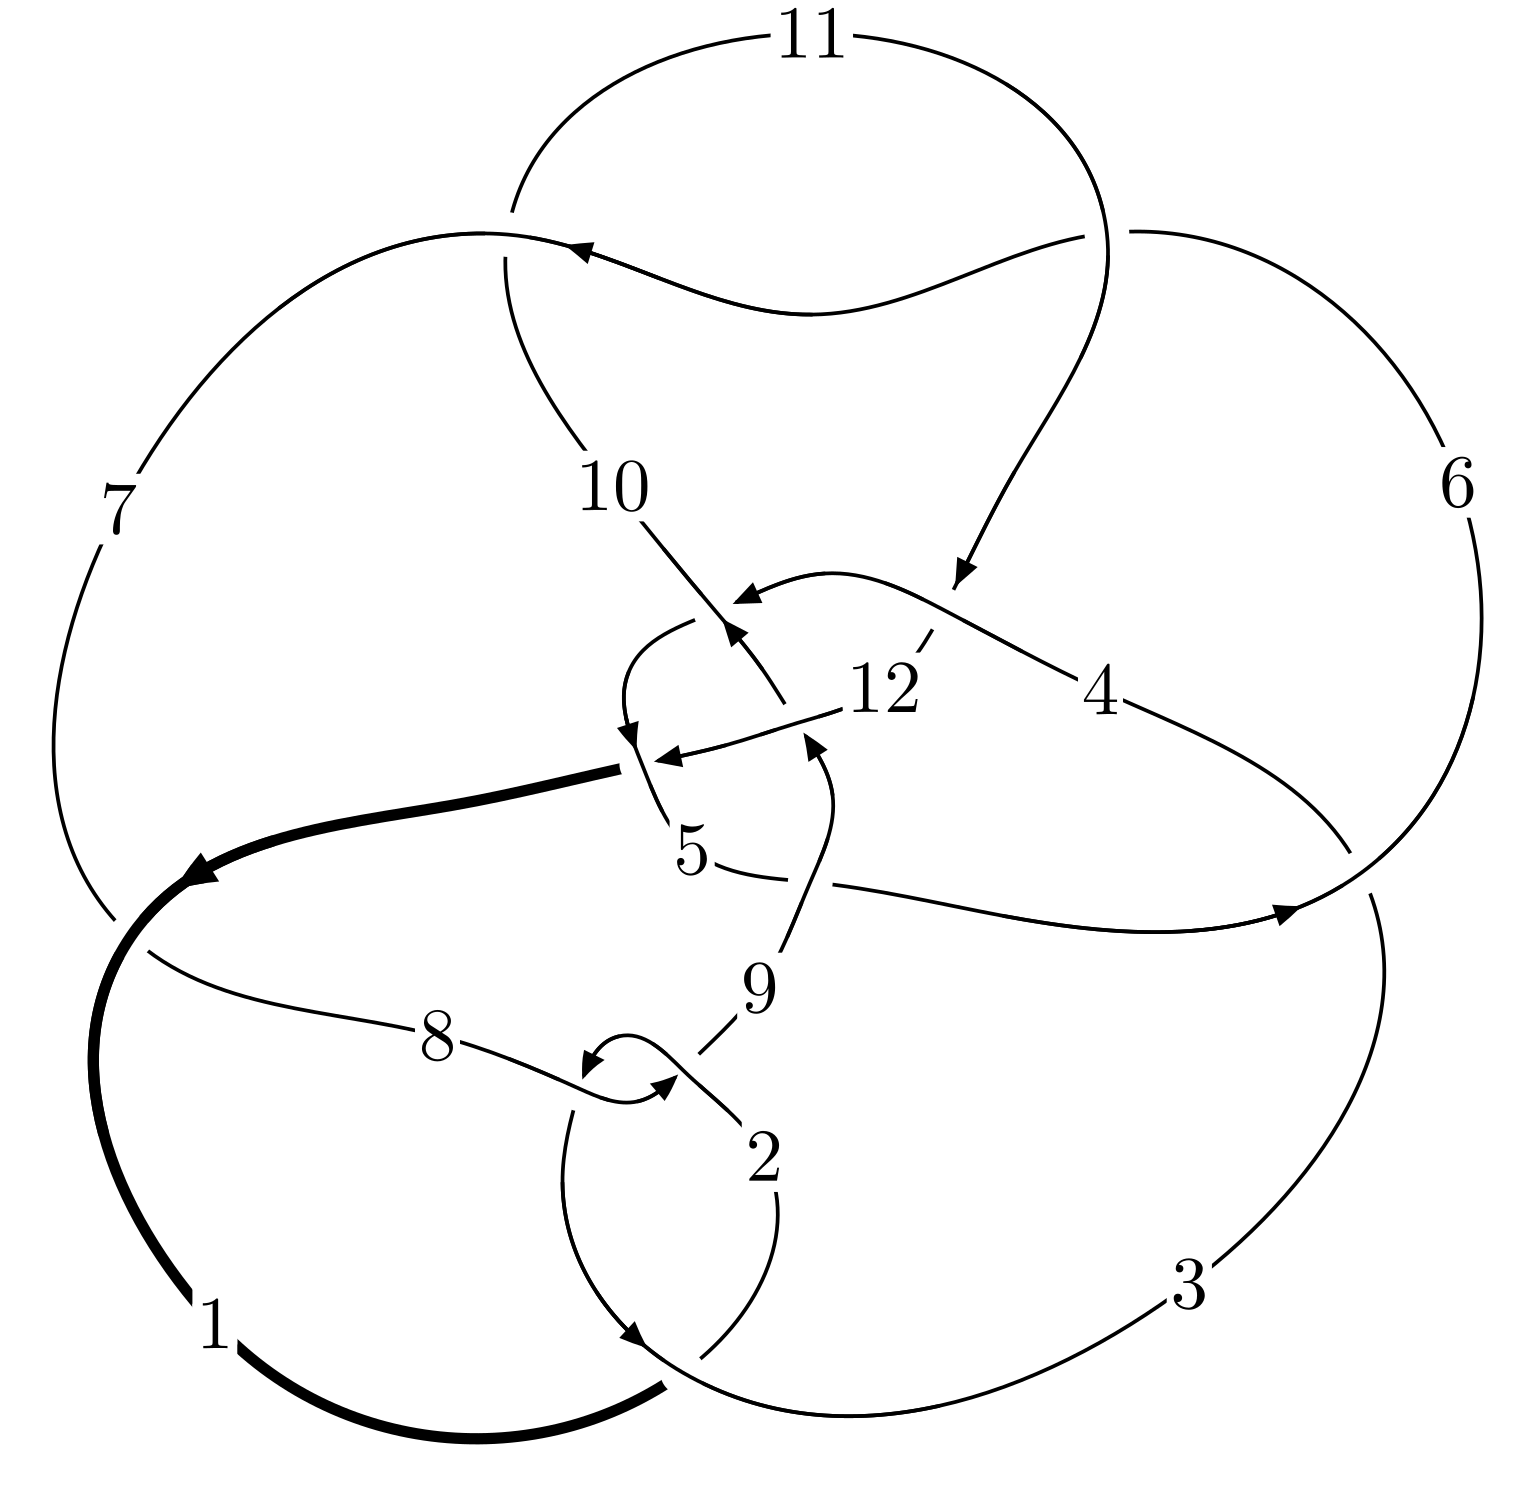
\includegraphics[width=112pt]{../../../GIT/diagram.site/Diagrams/png/1497_12a_0696.png}\\
\ \ \ A knot diagram\footnotemark}&
\allowdisplaybreaks
\textbf{Linearized knot diagam} \\
\cline{2-2}
 &
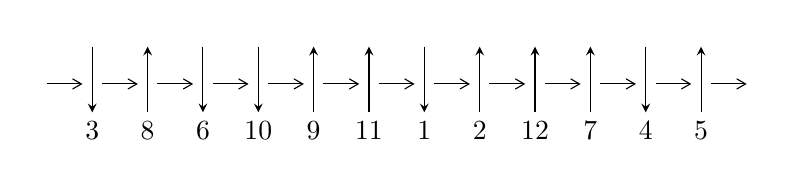
\begin{tikzpicture}[x=20pt, y=17pt]
	% nodes
	\node (C0) at (0, 0) {};
	\node (C1) at (1, 0) {};
	\node (C1U) at (1, +1) {};
	\node (C1D) at (1, -1) {3};

	\node (C2) at (2, 0) {};
	\node (C2U) at (2, +1) {};
	\node (C2D) at (2, -1) {8};

	\node (C3) at (3, 0) {};
	\node (C3U) at (3, +1) {};
	\node (C3D) at (3, -1) {6};

	\node (C4) at (4, 0) {};
	\node (C4U) at (4, +1) {};
	\node (C4D) at (4, -1) {10};

	\node (C5) at (5, 0) {};
	\node (C5U) at (5, +1) {};
	\node (C5D) at (5, -1) {9};

	\node (C6) at (6, 0) {};
	\node (C6U) at (6, +1) {};
	\node (C6D) at (6, -1) {11};

	\node (C7) at (7, 0) {};
	\node (C7U) at (7, +1) {};
	\node (C7D) at (7, -1) {1};

	\node (C8) at (8, 0) {};
	\node (C8U) at (8, +1) {};
	\node (C8D) at (8, -1) {2};

	\node (C9) at (9, 0) {};
	\node (C9U) at (9, +1) {};
	\node (C9D) at (9, -1) {12};

	\node (C10) at (10, 0) {};
	\node (C10U) at (10, +1) {};
	\node (C10D) at (10, -1) {7};

	\node (C11) at (11, 0) {};
	\node (C11U) at (11, +1) {};
	\node (C11D) at (11, -1) {4};

	\node (C12) at (12, 0) {};
	\node (C12U) at (12, +1) {};
	\node (C12D) at (12, -1) {5};
	\node (C13) at (13, 0) {};

	% arrows
	\draw[->,>={angle 60}]
	(C0) edge (C1) (C1) edge (C2) (C2) edge (C3) (C3) edge (C4) (C4) edge (C5) (C5) edge (C6) (C6) edge (C7) (C7) edge (C8) (C8) edge (C9) (C9) edge (C10) (C10) edge (C11) (C11) edge (C12) (C12) edge (C13) ;	\draw[->,>=stealth]
	(C1U) edge (C1D) (C2D) edge (C2U) (C3U) edge (C3D) (C4U) edge (C4D) (C5D) edge (C5U) (C6D) edge (C6U) (C7U) edge (C7D) (C8D) edge (C8U) (C9D) edge (C9U) (C10D) edge (C10U) (C11U) edge (C11D) (C12D) edge (C12U) ;
	\end{tikzpicture} \\
\hhline{~~} \\& 
\textbf{Solving Sequence} \\ \cline{2-2} 
 &
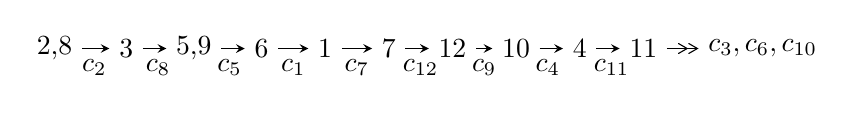
\begin{tikzpicture}[x=23pt, y=7pt]
	% node
	\node (A0) at (-1/8, 0) {2,8};
	\node (A1) at (1, 0) {3};
	\node (A2) at (33/16, 0) {5,9};
	\node (A3) at (25/8, 0) {6};
	\node (A4) at (33/8, 0) {1};
	\node (A5) at (41/8, 0) {7};
	\node (A6) at (49/8, 0) {12};
	\node (A7) at (57/8, 0) {10};
	\node (A8) at (65/8, 0) {4};
	\node (A9) at (73/8, 0) {11};
	\node (C1) at (1/2, -1) {$c_{2}$};
	\node (C2) at (3/2, -1) {$c_{8}$};
	\node (C3) at (21/8, -1) {$c_{5}$};
	\node (C4) at (29/8, -1) {$c_{1}$};
	\node (C5) at (37/8, -1) {$c_{7}$};
	\node (C6) at (45/8, -1) {$c_{12}$};
	\node (C7) at (53/8, -1) {$c_{9}$};
	\node (C8) at (61/8, -1) {$c_{4}$};
	\node (C9) at (69/8, -1) {$c_{11}$};
	\node (A10) at (11, 0) {$c_{3},c_{6},c_{10}$};

	% edge
	\draw[->,>=stealth]	
	(A0) edge (A1) (A1) edge (A2) (A2) edge (A3) (A3) edge (A4) (A4) edge (A5) (A5) edge (A6) (A6) edge (A7) (A7) edge (A8) (A8) edge (A9) ;
	\draw[->>,>={angle 60}]	
	(A9) edge (A10);
\end{tikzpicture} \\ 

\end{tabular} \\

\footnotetext{
The image of knot diagram is generated by the software ``\textbf{Draw programme}" developed by Andrew Bartholomew(\url{http://www.layer8.co.uk/maths/draw/index.htm\#Running-draw}), where we modified some parts for our purpose(\url{https://github.com/CATsTAILs/LinksPainter}).
}\phantom \\ \newline 
\centering \textbf{Ideals for irreducible components\footnotemark of $X_{\text{par}}$} 
 
\begin{align*}
I^u_{1}&=\langle 
1.41962\times10^{338} u^{180}-1.20195\times10^{338} u^{179}+\cdots+7.13962\times10^{336} b+2.76018\times10^{338},\\
\phantom{I^u_{1}}&\phantom{= \langle  }5.24278\times10^{338} u^{180}-3.50383\times10^{337} u^{179}+\cdots+7.13962\times10^{336} a-1.16139\times10^{339},\;u^{181}+46 u^{179}+\cdots- u-1\rangle \\
I^u_{2}&=\langle 
216 u^{42}-709 u^{41}+\cdots+131 b+943,\;347 u^{42}-1233 u^{41}+\cdots+131 a+2253,\;u^{43}- u^{42}+\cdots-7 u^2-1\rangle \\
\\
\end{align*}
\raggedright * 2 irreducible components of $\dim_{\mathbb{C}}=0$, with total 224 representations.\\
\footnotetext{All coefficients of polynomials are rational numbers. But the coefficients are sometimes approximated in decimal forms when there is not enough margin.}
\newpage
\renewcommand{\arraystretch}{1}
\centering \section*{I. $I^u_{1}= \langle 1.42\times10^{338} u^{180}-1.20\times10^{338} u^{179}+\cdots+7.14\times10^{336} b+2.76\times10^{338},\;5.24\times10^{338} u^{180}-3.50\times10^{337} u^{179}+\cdots+7.14\times10^{336} a-1.16\times10^{339},\;u^{181}+46 u^{179}+\cdots- u-1 \rangle$}
\flushleft \textbf{(i) Arc colorings}\\
\begin{tabular}{m{7pt} m{180pt} m{7pt} m{180pt} }
\flushright $a_{2}=$&$\begin{pmatrix}1\\0\end{pmatrix}$ \\
\flushright $a_{8}=$&$\begin{pmatrix}0\\u\end{pmatrix}$ \\
\flushright $a_{3}=$&$\begin{pmatrix}1\\- u^2\end{pmatrix}$ \\
\flushright $a_{5}=$&$\begin{pmatrix}-73.4323 u^{180}+4.90759 u^{179}+\cdots+95.1602 u+162.668\\-19.8838 u^{180}+16.8349 u^{179}+\cdots+143.589 u-38.6601\end{pmatrix}$ \\
\flushright $a_{9}=$&$\begin{pmatrix}u\\u\end{pmatrix}$ \\
\flushright $a_{6}=$&$\begin{pmatrix}-90.3427 u^{180}+13.4742 u^{179}+\cdots+160.636 u+174.596\\-36.7942 u^{180}+25.4015 u^{179}+\cdots+209.065 u-26.7327\end{pmatrix}$ \\
\flushright $a_{1}=$&$\begin{pmatrix}u^2+1\\- u^4\end{pmatrix}$ \\
\flushright $a_{7}=$&$\begin{pmatrix}u^5+2 u^3+u\\- u^7- u^5+u\end{pmatrix}$ \\
\flushright $a_{12}=$&$\begin{pmatrix}0.767022 u^{180}+10.6814 u^{179}+\cdots+5.72652 u-29.1072\\36.0408 u^{180}-10.4422 u^{179}+\cdots-136.012 u-31.3735\end{pmatrix}$ \\
\flushright $a_{10}=$&$\begin{pmatrix}-37.3943 u^{180}+24.9354 u^{179}+\cdots+178.969 u-20.9297\\51.2108 u^{180}-3.90059 u^{179}+\cdots-73.6166 u-109.969\end{pmatrix}$ \\
\flushright $a_{4}=$&$\begin{pmatrix}22.7530 u^{180}+7.33973 u^{179}+\cdots-20.3207 u-74.9072\\38.4414 u^{180}-8.59063 u^{179}+\cdots-122.749 u-47.7809\end{pmatrix}$ \\
\flushright $a_{11}=$&$\begin{pmatrix}-49.4226 u^{180}+30.0174 u^{179}+\cdots+232.737 u-21.1572\\43.4403 u^{180}+2.98078 u^{179}+\cdots-16.4521 u-126.279\end{pmatrix}$\\&\end{tabular}
\flushleft \textbf{(ii) Obstruction class $= -1$}\\~\\
\flushleft \textbf{(iii) Cusp Shapes $= -158.902 u^{180}+55.1634 u^{179}+\cdots+452.093 u+172.834$}\\~\\
\newpage\renewcommand{\arraystretch}{1}
\flushleft \textbf{(iv) u-Polynomials at the component}\newline \\
\begin{tabular}{m{50pt}|m{274pt}}
Crossings & \hspace{64pt}u-Polynomials at each crossing \\
\hline $$\begin{aligned}c_{1}\end{aligned}$$&$\begin{aligned}
&u^{181}+92 u^{180}+\cdots-15 u-1
\end{aligned}$\\
\hline $$\begin{aligned}c_{2},c_{8}\end{aligned}$$&$\begin{aligned}
&u^{181}+46 u^{179}+\cdots- u-1
\end{aligned}$\\
\hline $$\begin{aligned}c_{3}\end{aligned}$$&$\begin{aligned}
&u^{181}+13 u^{180}+\cdots+628733104 u-211700029
\end{aligned}$\\
\hline $$\begin{aligned}c_{4}\end{aligned}$$&$\begin{aligned}
&u^{181}- u^{180}+\cdots+212 u-3
\end{aligned}$\\
\hline $$\begin{aligned}c_{5}\end{aligned}$$&$\begin{aligned}
&u^{181}-4 u^{180}+\cdots-476890 u-36227
\end{aligned}$\\
\hline $$\begin{aligned}c_{6},c_{10}\end{aligned}$$&$\begin{aligned}
&u^{181}+u^{180}+\cdots+386176 u-88157
\end{aligned}$\\
\hline $$\begin{aligned}c_{7}\end{aligned}$$&$\begin{aligned}
&u^{181}-35 u^{179}+\cdots+202878969 u-21005497
\end{aligned}$\\
\hline $$\begin{aligned}c_{9}\end{aligned}$$&$\begin{aligned}
&u^{181}+14 u^{180}+\cdots-35 u-1
\end{aligned}$\\
\hline $$\begin{aligned}c_{11}\end{aligned}$$&$\begin{aligned}
&u^{181}+3 u^{180}+\cdots+1540072 u+1602889
\end{aligned}$\\
\hline $$\begin{aligned}c_{12}\end{aligned}$$&$\begin{aligned}
&u^{181}+2 u^{180}+\cdots+68 u+1
\end{aligned}$\\
\hline
\end{tabular}\\~\\
\newpage\renewcommand{\arraystretch}{1}
\flushleft \textbf{(v) Riley Polynomials at the component}\newline \\
\begin{tabular}{m{50pt}|m{274pt}}
Crossings & \hspace{64pt}Riley Polynomials at each crossing \\
\hline $$\begin{aligned}c_{1}\end{aligned}$$&$\begin{aligned}
&y^{181}+8 y^{180}+\cdots-87 y-1
\end{aligned}$\\
\hline $$\begin{aligned}c_{2},c_{8}\end{aligned}$$&$\begin{aligned}
&y^{181}+92 y^{180}+\cdots-15 y-1
\end{aligned}$\\
\hline $$\begin{aligned}c_{3}\end{aligned}$$&$\begin{aligned}
&y^{181}-61 y^{180}+\cdots+466437623685825210 y-44816902278600841
\end{aligned}$\\
\hline $$\begin{aligned}c_{4}\end{aligned}$$&$\begin{aligned}
&y^{181}-9 y^{180}+\cdots+17746 y-9
\end{aligned}$\\
\hline $$\begin{aligned}c_{5}\end{aligned}$$&$\begin{aligned}
&y^{181}+18 y^{180}+\cdots-14914777958 y-1312395529
\end{aligned}$\\
\hline $$\begin{aligned}c_{6},c_{10}\end{aligned}$$&$\begin{aligned}
&y^{181}+109 y^{180}+\cdots-436279416002 y-7771656649
\end{aligned}$\\
\hline $$\begin{aligned}c_{7}\end{aligned}$$&$\begin{aligned}
&y^{181}-70 y^{180}+\cdots+4677292519050717 y-441230904217009
\end{aligned}$\\
\hline $$\begin{aligned}c_{9}\end{aligned}$$&$\begin{aligned}
&y^{181}+2 y^{180}+\cdots-21 y-1
\end{aligned}$\\
\hline $$\begin{aligned}c_{11}\end{aligned}$$&$\begin{aligned}
&y^{181}-37 y^{180}+\cdots+210067324431820 y-2569253146321
\end{aligned}$\\
\hline $$\begin{aligned}c_{12}\end{aligned}$$&$\begin{aligned}
&y^{181}-2 y^{180}+\cdots+380 y-1
\end{aligned}$\\
\hline
\end{tabular}\\~\\
\newpage\flushleft \textbf{(vi) Complex Volumes and Cusp Shapes}
$$\begin{array}{c|c|c}  
\text{Solutions to }I^u_{1}& \I (\text{vol} + \sqrt{-1}CS) & \text{Cusp shape}\\
 \hline 
\begin{aligned}
u &= -0.595366 + 0.811631 I \\
a &= -0.220953 - 0.075715 I \\
b &= -0.254848 - 1.078240 I\end{aligned}
 & \phantom{-}2.02502 + 2.50091 I & \phantom{-0.000000 } 0 \\ \hline\begin{aligned}
u &= -0.595366 - 0.811631 I \\
a &= -0.220953 + 0.075715 I \\
b &= -0.254848 + 1.078240 I\end{aligned}
 & \phantom{-}2.02502 - 2.50091 I & \phantom{-0.000000 } 0 \\ \hline\begin{aligned}
u &= -0.634703 + 0.755237 I \\
a &= -0.579936 - 0.325735 I \\
b &= \phantom{-}0.693508 - 0.146741 I\end{aligned}
 & \phantom{-}2.19217 - 7.31387 I & \phantom{-0.000000 } 0 \\ \hline\begin{aligned}
u &= -0.634703 - 0.755237 I \\
a &= -0.579936 + 0.325735 I \\
b &= \phantom{-}0.693508 + 0.146741 I\end{aligned}
 & \phantom{-}2.19217 + 7.31387 I & \phantom{-0.000000 } 0 \\ \hline\begin{aligned}
u &= -0.370993 + 0.908742 I \\
a &= \phantom{-}1.62406 + 0.50872 I \\
b &= \phantom{-}1.62256 + 1.00947 I\end{aligned}
 & -3.48908 + 0.77709 I & \phantom{-0.000000 } 0 \\ \hline\begin{aligned}
u &= -0.370993 - 0.908742 I \\
a &= \phantom{-}1.62406 - 0.50872 I \\
b &= \phantom{-}1.62256 - 1.00947 I\end{aligned}
 & -3.48908 - 0.77709 I & \phantom{-0.000000 } 0 \\ \hline\begin{aligned}
u &= \phantom{-}0.704616 + 0.675912 I \\
a &= \phantom{-}0.1202880 - 0.0378242 I \\
b &= -0.807613 + 0.025109 I\end{aligned}
 & \phantom{-}2.13396 + 1.34395 I & \phantom{-0.000000 } 0 \\ \hline\begin{aligned}
u &= \phantom{-}0.704616 - 0.675912 I \\
a &= \phantom{-}0.1202880 + 0.0378242 I \\
b &= -0.807613 - 0.025109 I\end{aligned}
 & \phantom{-}2.13396 - 1.34395 I & \phantom{-0.000000 } 0 \\ \hline\begin{aligned}
u &= -0.561030 + 0.870578 I \\
a &= -0.412428 + 0.062081 I \\
b &= -1.139930 - 0.599033 I\end{aligned}
 & \phantom{-}3.28852 - 4.60568 I & \phantom{-0.000000 } 0 \\ \hline\begin{aligned}
u &= -0.561030 - 0.870578 I \\
a &= -0.412428 - 0.062081 I \\
b &= -1.139930 + 0.599033 I\end{aligned}
 & \phantom{-}3.28852 + 4.60568 I & \phantom{-0.000000 } 0\\
 \hline 
 \end{array}$$\newpage$$\begin{array}{c|c|c}  
\text{Solutions to }I^u_{1}& \I (\text{vol} + \sqrt{-1}CS) & \text{Cusp shape}\\
 \hline 
\begin{aligned}
u &= -0.123633 + 0.949947 I \\
a &= \phantom{-}1.157780 + 0.758066 I \\
b &= \phantom{-}1.192050 + 0.602453 I\end{aligned}
 & -3.65409 + 0.74327 I & \phantom{-0.000000 } 0 \\ \hline\begin{aligned}
u &= -0.123633 - 0.949947 I \\
a &= \phantom{-}1.157780 - 0.758066 I \\
b &= \phantom{-}1.192050 - 0.602453 I\end{aligned}
 & -3.65409 - 0.74327 I & \phantom{-0.000000 } 0 \\ \hline\begin{aligned}
u &= -0.892665 + 0.277974 I \\
a &= \phantom{-}0.309435 + 1.141240 I \\
b &= -0.237266 + 0.142966 I\end{aligned}
 & -2.75442 + 7.05989 I & \phantom{-0.000000 } 0 \\ \hline\begin{aligned}
u &= -0.892665 - 0.277974 I \\
a &= \phantom{-}0.309435 - 1.141240 I \\
b &= -0.237266 - 0.142966 I\end{aligned}
 & -2.75442 - 7.05989 I & \phantom{-0.000000 } 0 \\ \hline\begin{aligned}
u &= \phantom{-}0.746434 + 0.779550 I \\
a &= -0.411095 + 0.175466 I \\
b &= \phantom{-}0.750352 + 0.262441 I\end{aligned}
 & -1.22778 + 12.56300 I & \phantom{-0.000000 } 0 \\ \hline\begin{aligned}
u &= \phantom{-}0.746434 - 0.779550 I \\
a &= -0.411095 - 0.175466 I \\
b &= \phantom{-}0.750352 - 0.262441 I\end{aligned}
 & -1.22778 - 12.56300 I & \phantom{-0.000000 } 0 \\ \hline\begin{aligned}
u &= -0.908320 + 0.139101 I \\
a &= -0.360830 + 1.076450 I \\
b &= -0.288962 + 0.154564 I\end{aligned}
 & -5.95305 - 4.36779 I & \phantom{-0.000000 } 0 \\ \hline\begin{aligned}
u &= -0.908320 - 0.139101 I \\
a &= -0.360830 - 1.076450 I \\
b &= -0.288962 - 0.154564 I\end{aligned}
 & -5.95305 + 4.36779 I & \phantom{-0.000000 } 0 \\ \hline\begin{aligned}
u &= \phantom{-}0.886386 + 0.229234 I \\
a &= -0.22682 + 1.70159 I \\
b &= \phantom{-}0.059190 + 0.486908 I\end{aligned}
 & -1.18683 - 6.11657 I & \phantom{-0.000000 } 0 \\ \hline\begin{aligned}
u &= \phantom{-}0.886386 - 0.229234 I \\
a &= -0.22682 - 1.70159 I \\
b &= \phantom{-}0.059190 - 0.486908 I\end{aligned}
 & -1.18683 + 6.11657 I & \phantom{-0.000000 } 0\\
 \hline 
 \end{array}$$\newpage$$\begin{array}{c|c|c}  
\text{Solutions to }I^u_{1}& \I (\text{vol} + \sqrt{-1}CS) & \text{Cusp shape}\\
 \hline 
\begin{aligned}
u &= -0.863089 + 0.283405 I \\
a &= \phantom{-}0.28652 + 2.16697 I \\
b &= -0.284444 + 0.443997 I\end{aligned}
 & -4.1410 + 15.4470 I & \phantom{-0.000000 } 0 \\ \hline\begin{aligned}
u &= -0.863089 - 0.283405 I \\
a &= \phantom{-}0.28652 - 2.16697 I \\
b &= -0.284444 - 0.443997 I\end{aligned}
 & -4.1410 - 15.4470 I & \phantom{-0.000000 } 0 \\ \hline\begin{aligned}
u &= -0.358045 + 1.034350 I \\
a &= \phantom{-}2.59184 + 0.01919 I \\
b &= \phantom{-}2.80657 - 0.51443 I\end{aligned}
 & -3.60056 + 3.68982 I & \phantom{-0.000000 } 0 \\ \hline\begin{aligned}
u &= -0.358045 - 1.034350 I \\
a &= \phantom{-}2.59184 - 0.01919 I \\
b &= \phantom{-}2.80657 + 0.51443 I\end{aligned}
 & -3.60056 - 3.68982 I & \phantom{-0.000000 } 0 \\ \hline\begin{aligned}
u &= -0.551404 + 0.703655 I \\
a &= -0.250460 - 0.907719 I \\
b &= \phantom{-}0.456759 + 0.096369 I\end{aligned}
 & \phantom{-}3.77193 + 0.13944 I & \phantom{-0.000000 } 0 \\ \hline\begin{aligned}
u &= -0.551404 - 0.703655 I \\
a &= -0.250460 + 0.907719 I \\
b &= \phantom{-}0.456759 - 0.096369 I\end{aligned}
 & \phantom{-}3.77193 - 0.13944 I & \phantom{-0.000000 } 0 \\ \hline\begin{aligned}
u &= -0.459068 + 1.008750 I \\
a &= \phantom{-}2.20681 + 0.60195 I \\
b &= \phantom{-}3.63458 + 0.76309 I\end{aligned}
 & -2.44470 + 1.88493 I & \phantom{-0.000000 } 0 \\ \hline\begin{aligned}
u &= -0.459068 - 1.008750 I \\
a &= \phantom{-}2.20681 - 0.60195 I \\
b &= \phantom{-}3.63458 - 0.76309 I\end{aligned}
 & -2.44470 - 1.88493 I & \phantom{-0.000000 } 0 \\ \hline\begin{aligned}
u &= -0.518924 + 0.715548 I \\
a &= \phantom{-}0.77939 + 1.47033 I \\
b &= -0.523576 + 1.112090 I\end{aligned}
 & -3.08163 - 4.59143 I & \phantom{-0.000000 } 0 \\ \hline\begin{aligned}
u &= -0.518924 - 0.715548 I \\
a &= \phantom{-}0.77939 - 1.47033 I \\
b &= -0.523576 - 1.112090 I\end{aligned}
 & -3.08163 + 4.59143 I & \phantom{-0.000000 } 0\\
 \hline 
 \end{array}$$\newpage$$\begin{array}{c|c|c}  
\text{Solutions to }I^u_{1}& \I (\text{vol} + \sqrt{-1}CS) & \text{Cusp shape}\\
 \hline 
\begin{aligned}
u &= \phantom{-}0.157048 + 0.869008 I \\
a &= \phantom{-}0.148833 + 1.395630 I \\
b &= \phantom{-}0.829703 - 0.113133 I\end{aligned}
 & -3.37948 + 5.12393 I & \phantom{-0.000000 } 0 \\ \hline\begin{aligned}
u &= \phantom{-}0.157048 - 0.869008 I \\
a &= \phantom{-}0.148833 - 1.395630 I \\
b &= \phantom{-}0.829703 + 0.113133 I\end{aligned}
 & -3.37948 - 5.12393 I & \phantom{-0.000000 } 0 \\ \hline\begin{aligned}
u &= \phantom{-}0.801141 + 0.348018 I \\
a &= \phantom{-}0.83475 + 1.18270 I \\
b &= \phantom{-}0.235543 - 0.110065 I\end{aligned}
 & -3.70946 - 1.31308 I & \phantom{-0.000000 } 0 \\ \hline\begin{aligned}
u &= \phantom{-}0.801141 - 0.348018 I \\
a &= \phantom{-}0.83475 - 1.18270 I \\
b &= \phantom{-}0.235543 + 0.110065 I\end{aligned}
 & -3.70946 + 1.31308 I & \phantom{-0.000000 } 0 \\ \hline\begin{aligned}
u &= \phantom{-}0.742863 + 0.849193 I \\
a &= -0.178981 - 0.043073 I \\
b &= \phantom{-}0.014625 + 0.869414 I\end{aligned}
 & -1.41715 - 6.99847 I & \phantom{-0.000000 } 0 \\ \hline\begin{aligned}
u &= \phantom{-}0.742863 - 0.849193 I \\
a &= -0.178981 + 0.043073 I \\
b &= \phantom{-}0.014625 - 0.869414 I\end{aligned}
 & -1.41715 + 6.99847 I & \phantom{-0.000000 } 0 \\ \hline\begin{aligned}
u &= \phantom{-}0.503467 + 1.013000 I \\
a &= \phantom{-}0.077435 - 0.434592 I \\
b &= \phantom{-}0.038806 - 1.403750 I\end{aligned}
 & -0.24505 + 2.88016 I & \phantom{-0.000000 } 0 \\ \hline\begin{aligned}
u &= \phantom{-}0.503467 - 1.013000 I \\
a &= \phantom{-}0.077435 + 0.434592 I \\
b &= \phantom{-}0.038806 + 1.403750 I\end{aligned}
 & -0.24505 - 2.88016 I & \phantom{-0.000000 } 0 \\ \hline\begin{aligned}
u &= \phantom{-}0.440356 + 1.048290 I \\
a &= -0.998995 - 0.403249 I \\
b &= -1.63920 - 1.06547 I\end{aligned}
 & -0.56992 + 2.55721 I & \phantom{-0.000000 } 0 \\ \hline\begin{aligned}
u &= \phantom{-}0.440356 - 1.048290 I \\
a &= -0.998995 + 0.403249 I \\
b &= -1.63920 + 1.06547 I\end{aligned}
 & -0.56992 - 2.55721 I & \phantom{-0.000000 } 0\\
 \hline 
 \end{array}$$\newpage$$\begin{array}{c|c|c}  
\text{Solutions to }I^u_{1}& \I (\text{vol} + \sqrt{-1}CS) & \text{Cusp shape}\\
 \hline 
\begin{aligned}
u &= \phantom{-}0.675539 + 0.915043 I \\
a &= -0.025051 + 0.332177 I \\
b &= \phantom{-}0.076457 - 0.316468 I\end{aligned}
 & \phantom{-}1.44991 + 3.88925 I & \phantom{-0.000000 } 0 \\ \hline\begin{aligned}
u &= \phantom{-}0.675539 - 0.915043 I \\
a &= -0.025051 - 0.332177 I \\
b &= \phantom{-}0.076457 + 0.316468 I\end{aligned}
 & \phantom{-}1.44991 - 3.88925 I & \phantom{-0.000000 } 0 \\ \hline\begin{aligned}
u &= -0.412926 + 1.060430 I \\
a &= \phantom{-}1.37075 + 0.99233 I \\
b &= \phantom{-}2.27954 + 0.39999 I\end{aligned}
 & -5.20267 - 0.90227 I & \phantom{-0.000000 } 0 \\ \hline\begin{aligned}
u &= -0.412926 - 1.060430 I \\
a &= \phantom{-}1.37075 - 0.99233 I \\
b &= \phantom{-}2.27954 - 0.39999 I\end{aligned}
 & -5.20267 + 0.90227 I & \phantom{-0.000000 } 0 \\ \hline\begin{aligned}
u &= \phantom{-}0.861028\phantom{ +0.000000I} \\
a &= \phantom{-}0.988370\phantom{ +0.000000I} \\
b &= -0.0890765\phantom{ +0.000000I}\end{aligned}
 & \phantom{-}1.61341\phantom{ +0.000000I} & \phantom{-0.000000 } 0 \\ \hline\begin{aligned}
u &= -0.233629 + 1.126220 I \\
a &= \phantom{-}1.55018 + 0.13866 I \\
b &= \phantom{-}2.41784 - 0.39138 I\end{aligned}
 & -4.23044 + 0.97702 I & \phantom{-0.000000 } 0 \\ \hline\begin{aligned}
u &= -0.233629 - 1.126220 I \\
a &= \phantom{-}1.55018 - 0.13866 I \\
b &= \phantom{-}2.41784 + 0.39138 I\end{aligned}
 & -4.23044 - 0.97702 I & \phantom{-0.000000 } 0 \\ \hline\begin{aligned}
u &= -0.780080 + 0.325656 I \\
a &= -0.09035 - 2.02154 I \\
b &= \phantom{-}0.147982 - 0.615166 I\end{aligned}
 & \phantom{-}0.37862 + 3.76264 I & \phantom{-0.000000 } 0 \\ \hline\begin{aligned}
u &= -0.780080 - 0.325656 I \\
a &= -0.09035 + 2.02154 I \\
b &= \phantom{-}0.147982 + 0.615166 I\end{aligned}
 & \phantom{-}0.37862 - 3.76264 I & \phantom{-0.000000 } 0 \\ \hline\begin{aligned}
u &= \phantom{-}0.804821 + 0.255351 I \\
a &= \phantom{-}0.44956 - 2.29525 I \\
b &= -0.157892 - 0.433264 I\end{aligned}
 & -0.38569 - 9.16610 I & \phantom{-0.000000 } 0\\
 \hline 
 \end{array}$$\newpage$$\begin{array}{c|c|c}  
\text{Solutions to }I^u_{1}& \I (\text{vol} + \sqrt{-1}CS) & \text{Cusp shape}\\
 \hline 
\begin{aligned}
u &= \phantom{-}0.804821 - 0.255351 I \\
a &= \phantom{-}0.44956 + 2.29525 I \\
b &= -0.157892 + 0.433264 I\end{aligned}
 & -0.38569 + 9.16610 I & \phantom{-0.000000 } 0 \\ \hline\begin{aligned}
u &= -0.345041 + 1.103590 I \\
a &= \phantom{-}1.14839 + 0.91569 I \\
b &= \phantom{-}1.98156 + 0.52442 I\end{aligned}
 & -5.24590 - 1.12386 I & \phantom{-0.000000 } 0 \\ \hline\begin{aligned}
u &= -0.345041 - 1.103590 I \\
a &= \phantom{-}1.14839 - 0.91569 I \\
b &= \phantom{-}1.98156 - 0.52442 I\end{aligned}
 & -5.24590 + 1.12386 I & \phantom{-0.000000 } 0 \\ \hline\begin{aligned}
u &= \phantom{-}0.547805 + 1.019380 I \\
a &= \phantom{-}0.784206 + 0.544874 I \\
b &= \phantom{-}0.841813 - 0.555541 I\end{aligned}
 & -1.081600 + 0.205365 I & \phantom{-0.000000 } 0 \\ \hline\begin{aligned}
u &= \phantom{-}0.547805 - 1.019380 I \\
a &= \phantom{-}0.784206 - 0.544874 I \\
b &= \phantom{-}0.841813 + 0.555541 I\end{aligned}
 & -1.081600 - 0.205365 I & \phantom{-0.000000 } 0 \\ \hline\begin{aligned}
u &= -0.646682 + 0.534024 I \\
a &= \phantom{-}1.06485 - 1.03858 I \\
b &= \phantom{-}0.573543 + 0.171316 I\end{aligned}
 & -2.55016 + 1.06949 I & \phantom{-0.000000 } 0 \\ \hline\begin{aligned}
u &= -0.646682 - 0.534024 I \\
a &= \phantom{-}1.06485 + 1.03858 I \\
b &= \phantom{-}0.573543 - 0.171316 I\end{aligned}
 & -2.55016 - 1.06949 I & \phantom{-0.000000 } 0 \\ \hline\begin{aligned}
u &= -0.332377 + 0.769653 I \\
a &= -0.21601 + 2.30748 I \\
b &= -0.33659 + 2.64018 I\end{aligned}
 & -2.68713 - 6.41286 I & \phantom{-0.000000 } 0 \\ \hline\begin{aligned}
u &= -0.332377 - 0.769653 I \\
a &= -0.21601 - 2.30748 I \\
b &= -0.33659 - 2.64018 I\end{aligned}
 & -2.68713 + 6.41286 I & \phantom{-0.000000 } 0 \\ \hline\begin{aligned}
u &= \phantom{-}0.725805 + 0.415106 I \\
a &= -0.606486 - 0.116539 I \\
b &= -0.589604 + 0.253650 I\end{aligned}
 & \phantom{-}0.362740 + 1.324350 I & \phantom{-0.000000 } 0\\
 \hline 
 \end{array}$$\newpage$$\begin{array}{c|c|c}  
\text{Solutions to }I^u_{1}& \I (\text{vol} + \sqrt{-1}CS) & \text{Cusp shape}\\
 \hline 
\begin{aligned}
u &= \phantom{-}0.725805 - 0.415106 I \\
a &= -0.606486 + 0.116539 I \\
b &= -0.589604 - 0.253650 I\end{aligned}
 & \phantom{-}0.362740 - 1.324350 I & \phantom{-0.000000 } 0 \\ \hline\begin{aligned}
u &= -0.116898 + 1.158270 I \\
a &= \phantom{-}1.53679 + 0.17839 I \\
b &= \phantom{-}2.32806 - 0.08252 I\end{aligned}
 & -4.25718 + 1.20520 I & \phantom{-0.000000 } 0 \\ \hline\begin{aligned}
u &= -0.116898 - 1.158270 I \\
a &= \phantom{-}1.53679 - 0.17839 I \\
b &= \phantom{-}2.32806 + 0.08252 I\end{aligned}
 & -4.25718 - 1.20520 I & \phantom{-0.000000 } 0 \\ \hline\begin{aligned}
u &= \phantom{-}0.383159 + 1.103090 I \\
a &= -0.962500 + 0.752145 I \\
b &= -1.77229 + 2.36253 I\end{aligned}
 & -5.30848 - 3.20886 I & \phantom{-0.000000 } 0 \\ \hline\begin{aligned}
u &= \phantom{-}0.383159 - 1.103090 I \\
a &= -0.962500 - 0.752145 I \\
b &= -1.77229 - 2.36253 I\end{aligned}
 & -5.30848 + 3.20886 I & \phantom{-0.000000 } 0 \\ \hline\begin{aligned}
u &= -0.451440 + 1.080940 I \\
a &= \phantom{-}0.800482 - 0.588323 I \\
b &= \phantom{-}0.938164 + 0.472350 I\end{aligned}
 & -1.163910 - 0.786720 I & \phantom{-0.000000 } 0 \\ \hline\begin{aligned}
u &= -0.451440 - 1.080940 I \\
a &= \phantom{-}0.800482 + 0.588323 I \\
b &= \phantom{-}0.938164 - 0.472350 I\end{aligned}
 & -1.163910 + 0.786720 I & \phantom{-0.000000 } 0 \\ \hline\begin{aligned}
u &= \phantom{-}0.422902 + 1.098430 I \\
a &= \phantom{-}1.84201 + 0.78115 I \\
b &= \phantom{-}2.20323 + 1.08182 I\end{aligned}
 & -2.23070 + 0.56794 I & \phantom{-0.000000 } 0 \\ \hline\begin{aligned}
u &= \phantom{-}0.422902 - 1.098430 I \\
a &= \phantom{-}1.84201 - 0.78115 I \\
b &= \phantom{-}2.20323 - 1.08182 I\end{aligned}
 & -2.23070 - 0.56794 I & \phantom{-0.000000 } 0 \\ \hline\begin{aligned}
u &= -0.458491 + 1.084610 I \\
a &= -0.714432 - 1.185340 I \\
b &= -1.32638 - 3.18509 I\end{aligned}
 & \phantom{-}0.40177 - 3.55687 I & \phantom{-0.000000 } 0\\
 \hline 
 \end{array}$$\newpage$$\begin{array}{c|c|c}  
\text{Solutions to }I^u_{1}& \I (\text{vol} + \sqrt{-1}CS) & \text{Cusp shape}\\
 \hline 
\begin{aligned}
u &= -0.458491 - 1.084610 I \\
a &= -0.714432 + 1.185340 I \\
b &= -1.32638 + 3.18509 I\end{aligned}
 & \phantom{-}0.40177 + 3.55687 I & \phantom{-0.000000 } 0 \\ \hline\begin{aligned}
u &= -0.469416 + 1.082820 I \\
a &= -0.093041 - 0.551849 I \\
b &= \phantom{-}0.247775 + 0.351022 I\end{aligned}
 & -1.03527 - 6.27958 I & \phantom{-0.000000 } 0 \\ \hline\begin{aligned}
u &= -0.469416 - 1.082820 I \\
a &= -0.093041 + 0.551849 I \\
b &= \phantom{-}0.247775 - 0.351022 I\end{aligned}
 & -1.03527 + 6.27958 I & \phantom{-0.000000 } 0 \\ \hline\begin{aligned}
u &= \phantom{-}0.233183 + 1.157760 I \\
a &= \phantom{-}0.917580 - 0.478336 I \\
b &= \phantom{-}2.19796 - 0.42643 I\end{aligned}
 & -8.46939 + 1.54159 I & \phantom{-0.000000 } 0 \\ \hline\begin{aligned}
u &= \phantom{-}0.233183 - 1.157760 I \\
a &= \phantom{-}0.917580 + 0.478336 I \\
b &= \phantom{-}2.19796 + 0.42643 I\end{aligned}
 & -8.46939 - 1.54159 I & \phantom{-0.000000 } 0 \\ \hline\begin{aligned}
u &= -0.798609 + 0.127641 I \\
a &= \phantom{-}0.80609 + 1.99177 I \\
b &= -0.098263 + 0.236236 I\end{aligned}
 & -6.25329 + 3.52327 I & \phantom{-0.000000 } 0 \\ \hline\begin{aligned}
u &= -0.798609 - 0.127641 I \\
a &= \phantom{-}0.80609 - 1.99177 I \\
b &= -0.098263 - 0.236236 I\end{aligned}
 & -6.25329 - 3.52327 I & \phantom{-0.000000 } 0 \\ \hline\begin{aligned}
u &= -0.549070 + 1.059660 I \\
a &= -1.19056 + 1.02991 I \\
b &= -2.13444 + 1.17123 I\end{aligned}
 & -4.17076 - 5.74669 I & \phantom{-0.000000 } 0 \\ \hline\begin{aligned}
u &= -0.549070 - 1.059660 I \\
a &= -1.19056 - 1.02991 I \\
b &= -2.13444 - 1.17123 I\end{aligned}
 & -4.17076 + 5.74669 I & \phantom{-0.000000 } 0 \\ \hline\begin{aligned}
u &= \phantom{-}0.482657 + 1.093120 I \\
a &= \phantom{-}1.76141 - 0.62048 I \\
b &= \phantom{-}3.01916 - 1.13238 I\end{aligned}
 & -0.10816 + 4.41774 I & \phantom{-0.000000 } 0\\
 \hline 
 \end{array}$$\newpage$$\begin{array}{c|c|c}  
\text{Solutions to }I^u_{1}& \I (\text{vol} + \sqrt{-1}CS) & \text{Cusp shape}\\
 \hline 
\begin{aligned}
u &= \phantom{-}0.482657 - 1.093120 I \\
a &= \phantom{-}1.76141 + 0.62048 I \\
b &= \phantom{-}3.01916 + 1.13238 I\end{aligned}
 & -0.10816 - 4.41774 I & \phantom{-0.000000 } 0 \\ \hline\begin{aligned}
u &= -0.824240 + 0.867010 I \\
a &= -0.033092 - 0.182100 I \\
b &= -0.441577 + 0.091360 I\end{aligned}
 & \phantom{-}3.03707 - 3.05245 I & \phantom{-0.000000 } 0 \\ \hline\begin{aligned}
u &= -0.824240 - 0.867010 I \\
a &= -0.033092 + 0.182100 I \\
b &= -0.441577 - 0.091360 I\end{aligned}
 & \phantom{-}3.03707 + 3.05245 I & \phantom{-0.000000 } 0 \\ \hline\begin{aligned}
u &= \phantom{-}0.601604 + 1.035200 I \\
a &= -0.097785 + 0.631510 I \\
b &= \phantom{-}0.348734 + 0.413731 I\end{aligned}
 & -1.38718 + 3.71905 I & \phantom{-0.000000 } 0 \\ \hline\begin{aligned}
u &= \phantom{-}0.601604 - 1.035200 I \\
a &= -0.097785 - 0.631510 I \\
b &= \phantom{-}0.348734 - 0.413731 I\end{aligned}
 & -1.38718 - 3.71905 I & \phantom{-0.000000 } 0 \\ \hline\begin{aligned}
u &= -0.542572 + 1.070150 I \\
a &= -1.78926 + 0.50083 I \\
b &= -2.97774 + 0.92695 I\end{aligned}
 & -1.49183 - 7.86123 I & \phantom{-0.000000 } 0 \\ \hline\begin{aligned}
u &= -0.542572 - 1.070150 I \\
a &= -1.78926 - 0.50083 I \\
b &= -2.97774 - 0.92695 I\end{aligned}
 & -1.49183 + 7.86123 I & \phantom{-0.000000 } 0 \\ \hline\begin{aligned}
u &= \phantom{-}0.309993 + 1.159420 I \\
a &= \phantom{-}1.404010 + 0.151915 I \\
b &= \phantom{-}2.42155 + 1.36019 I\end{aligned}
 & -9.30742 - 2.43693 I & \phantom{-0.000000 } 0 \\ \hline\begin{aligned}
u &= \phantom{-}0.309993 - 1.159420 I \\
a &= \phantom{-}1.404010 - 0.151915 I \\
b &= \phantom{-}2.42155 - 1.36019 I\end{aligned}
 & -9.30742 + 2.43693 I & \phantom{-0.000000 } 0 \\ \hline\begin{aligned}
u &= \phantom{-}0.289712 + 0.743814 I \\
a &= -0.063647 - 0.935766 I \\
b &= -0.344138 - 1.281830 I\end{aligned}
 & -0.22312 + 2.03344 I & \phantom{-0.000000 } 0\\
 \hline 
 \end{array}$$\newpage$$\begin{array}{c|c|c}  
\text{Solutions to }I^u_{1}& \I (\text{vol} + \sqrt{-1}CS) & \text{Cusp shape}\\
 \hline 
\begin{aligned}
u &= \phantom{-}0.289712 - 0.743814 I \\
a &= -0.063647 + 0.935766 I \\
b &= -0.344138 + 1.281830 I\end{aligned}
 & -0.22312 - 2.03344 I & \phantom{-0.000000 } 0 \\ \hline\begin{aligned}
u &= \phantom{-}0.616770 + 0.505046 I \\
a &= \phantom{-}0.197342 - 0.798565 I \\
b &= -1.308510 - 0.474613 I\end{aligned}
 & \phantom{-}0.41886 + 4.40049 I & \phantom{-0.000000 } 0 \\ \hline\begin{aligned}
u &= \phantom{-}0.616770 - 0.505046 I \\
a &= \phantom{-}0.197342 + 0.798565 I \\
b &= -1.308510 + 0.474613 I\end{aligned}
 & \phantom{-}0.41886 - 4.40049 I & \phantom{-0.000000 } 0 \\ \hline\begin{aligned}
u &= \phantom{-}0.580502 + 0.544023 I \\
a &= \phantom{-}0.967205 + 0.116282 I \\
b &= -0.422730 - 0.119944 I\end{aligned}
 & \phantom{-}1.13183 + 1.44638 I & \phantom{-0.000000 } 0 \\ \hline\begin{aligned}
u &= \phantom{-}0.580502 - 0.544023 I \\
a &= \phantom{-}0.967205 - 0.116282 I \\
b &= -0.422730 + 0.119944 I\end{aligned}
 & \phantom{-}1.13183 - 1.44638 I & \phantom{-0.000000 } 0 \\ \hline\begin{aligned}
u &= \phantom{-}0.473790 + 1.108350 I \\
a &= -2.09192 + 1.01004 I \\
b &= -2.83871 + 1.11234 I\end{aligned}
 & -1.86361 + 6.85669 I & \phantom{-0.000000 } 0 \\ \hline\begin{aligned}
u &= \phantom{-}0.473790 - 1.108350 I \\
a &= -2.09192 - 1.01004 I \\
b &= -2.83871 - 1.11234 I\end{aligned}
 & -1.86361 - 6.85669 I & \phantom{-0.000000 } 0 \\ \hline\begin{aligned}
u &= \phantom{-}0.420548 + 1.130940 I \\
a &= -1.58806 - 0.83622 I \\
b &= -2.47273 - 0.52937 I\end{aligned}
 & -7.22191 + 1.52317 I & \phantom{-0.000000 } 0 \\ \hline\begin{aligned}
u &= \phantom{-}0.420548 - 1.130940 I \\
a &= -1.58806 + 0.83622 I \\
b &= -2.47273 + 0.52937 I\end{aligned}
 & -7.22191 - 1.52317 I & \phantom{-0.000000 } 0 \\ \hline\begin{aligned}
u &= -0.541223 + 1.084210 I \\
a &= -1.257890 + 0.093994 I \\
b &= -1.63526 + 0.44936 I\end{aligned}
 & -1.74817 - 7.28829 I & \phantom{-0.000000 } 0\\
 \hline 
 \end{array}$$\newpage$$\begin{array}{c|c|c}  
\text{Solutions to }I^u_{1}& \I (\text{vol} + \sqrt{-1}CS) & \text{Cusp shape}\\
 \hline 
\begin{aligned}
u &= -0.541223 - 1.084210 I \\
a &= -1.257890 - 0.093994 I \\
b &= -1.63526 - 0.44936 I\end{aligned}
 & -1.74817 + 7.28829 I & \phantom{-0.000000 } 0 \\ \hline\begin{aligned}
u &= \phantom{-}0.236625 + 1.188870 I \\
a &= -0.299425 + 0.548056 I \\
b &= -0.961238 + 0.363852 I\end{aligned}
 & -4.48456 + 4.02067 I & \phantom{-0.000000 } 0 \\ \hline\begin{aligned}
u &= \phantom{-}0.236625 - 1.188870 I \\
a &= -0.299425 - 0.548056 I \\
b &= -0.961238 - 0.363852 I\end{aligned}
 & -4.48456 - 4.02067 I & \phantom{-0.000000 } 0 \\ \hline\begin{aligned}
u &= \phantom{-}0.747874 + 0.244536 I \\
a &= -0.46227 + 2.50916 I \\
b &= \phantom{-}0.563510 + 0.429958 I\end{aligned}
 & -5.13314 - 5.71116 I & \phantom{-0.000000 } 0 \\ \hline\begin{aligned}
u &= \phantom{-}0.747874 - 0.244536 I \\
a &= -0.46227 - 2.50916 I \\
b &= \phantom{-}0.563510 - 0.429958 I\end{aligned}
 & -5.13314 + 5.71116 I & \phantom{-0.000000 } 0 \\ \hline\begin{aligned}
u &= -0.675870 + 0.399177 I \\
a &= \phantom{-}0.50445 - 2.05809 I \\
b &= \phantom{-}0.071628 - 0.414562 I\end{aligned}
 & \phantom{-}0.45098 + 3.15192 I & \phantom{-0.000000 } 0 \\ \hline\begin{aligned}
u &= -0.675870 - 0.399177 I \\
a &= \phantom{-}0.50445 + 2.05809 I \\
b &= \phantom{-}0.071628 + 0.414562 I\end{aligned}
 & \phantom{-}0.45098 - 3.15192 I & \phantom{-0.000000 } 0 \\ \hline\begin{aligned}
u &= -0.535036 + 1.094650 I \\
a &= -2.61029 - 0.28492 I \\
b &= -3.42078 - 0.57740 I\end{aligned}
 & -2.23095 - 10.64040 I & \phantom{-0.000000 } 0 \\ \hline\begin{aligned}
u &= -0.535036 - 1.094650 I \\
a &= -2.61029 + 0.28492 I \\
b &= -3.42078 + 0.57740 I\end{aligned}
 & -2.23095 + 10.64040 I & \phantom{-0.000000 } 0 \\ \hline\begin{aligned}
u &= \phantom{-}0.473276 + 1.129650 I \\
a &= \phantom{-}1.087770 - 0.548024 I \\
b &= \phantom{-}1.80572 + 0.27444 I\end{aligned}
 & -6.84995 + 6.27359 I & \phantom{-0.000000 } 0\\
 \hline 
 \end{array}$$\newpage$$\begin{array}{c|c|c}  
\text{Solutions to }I^u_{1}& \I (\text{vol} + \sqrt{-1}CS) & \text{Cusp shape}\\
 \hline 
\begin{aligned}
u &= \phantom{-}0.473276 - 1.129650 I \\
a &= \phantom{-}1.087770 + 0.548024 I \\
b &= \phantom{-}1.80572 - 0.27444 I\end{aligned}
 & -6.84995 - 6.27359 I & \phantom{-0.000000 } 0 \\ \hline\begin{aligned}
u &= \phantom{-}0.762848 + 0.135949 I \\
a &= \phantom{-}0.58678 + 1.57032 I \\
b &= \phantom{-}0.882411 + 0.656826 I\end{aligned}
 & -5.01247 - 6.00479 I & \phantom{-0.000000 } 0 \\ \hline\begin{aligned}
u &= \phantom{-}0.762848 - 0.135949 I \\
a &= \phantom{-}0.58678 - 1.57032 I \\
b &= \phantom{-}0.882411 - 0.656826 I\end{aligned}
 & -5.01247 + 6.00479 I & \phantom{-0.000000 } 0 \\ \hline\begin{aligned}
u &= \phantom{-}0.502601 + 1.119240 I \\
a &= -0.240995 + 1.042730 I \\
b &= -0.37286 + 2.90419 I\end{aligned}
 & -4.45118 + 10.75730 I & \phantom{-0.000000 } 0 \\ \hline\begin{aligned}
u &= \phantom{-}0.502601 - 1.119240 I \\
a &= -0.240995 - 1.042730 I \\
b &= -0.37286 - 2.90419 I\end{aligned}
 & -4.45118 - 10.75730 I & \phantom{-0.000000 } 0 \\ \hline\begin{aligned}
u &= \phantom{-}0.287541 + 1.193830 I \\
a &= -1.48803 - 0.36873 I \\
b &= -2.46237 - 1.21265 I\end{aligned}
 & -4.89969 - 5.76769 I & \phantom{-0.000000 } 0 \\ \hline\begin{aligned}
u &= \phantom{-}0.287541 - 1.193830 I \\
a &= -1.48803 + 0.36873 I \\
b &= -2.46237 + 1.21265 I\end{aligned}
 & -4.89969 + 5.76769 I & \phantom{-0.000000 } 0 \\ \hline\begin{aligned}
u &= -0.496681 + 1.123250 I \\
a &= -1.58307 + 0.85958 I \\
b &= -2.33142 + 0.80238 I\end{aligned}
 & -4.27542 - 6.44833 I & \phantom{-0.000000 } 0 \\ \hline\begin{aligned}
u &= -0.496681 - 1.123250 I \\
a &= -1.58307 - 0.85958 I \\
b &= -2.33142 - 0.80238 I\end{aligned}
 & -4.27542 + 6.44833 I & \phantom{-0.000000 } 0 \\ \hline\begin{aligned}
u &= -0.657010 + 0.372835 I \\
a &= \phantom{-}0.280475 - 1.137390 I \\
b &= -0.122076 - 0.598640 I\end{aligned}
 & \phantom{-}0.30441 + 2.61964 I & \phantom{-0.000000 } 0\\
 \hline 
 \end{array}$$\newpage$$\begin{array}{c|c|c}  
\text{Solutions to }I^u_{1}& \I (\text{vol} + \sqrt{-1}CS) & \text{Cusp shape}\\
 \hline 
\begin{aligned}
u &= -0.657010 - 0.372835 I \\
a &= \phantom{-}0.280475 + 1.137390 I \\
b &= -0.122076 + 0.598640 I\end{aligned}
 & \phantom{-}0.30441 - 2.61964 I & \phantom{-0.000000 } 0 \\ \hline\begin{aligned}
u &= \phantom{-}0.898188 + 0.863137 I \\
a &= -0.164321 + 0.120590 I \\
b &= \phantom{-}0.048251 + 0.216107 I\end{aligned}
 & \phantom{-}0.87736 + 3.27537 I & \phantom{-0.000000 } 0 \\ \hline\begin{aligned}
u &= \phantom{-}0.898188 - 0.863137 I \\
a &= -0.164321 - 0.120590 I \\
b &= \phantom{-}0.048251 - 0.216107 I\end{aligned}
 & \phantom{-}0.87736 - 3.27537 I & \phantom{-0.000000 } 0 \\ \hline\begin{aligned}
u &= -0.650324 + 0.362682 I \\
a &= -0.40903 - 2.59114 I \\
b &= \phantom{-}0.197113 - 1.304150 I\end{aligned}
 & -0.10346 + 6.00550 I & \phantom{-0.000000 } 0 \\ \hline\begin{aligned}
u &= -0.650324 - 0.362682 I \\
a &= -0.40903 + 2.59114 I \\
b &= \phantom{-}0.197113 + 1.304150 I\end{aligned}
 & -0.10346 - 6.00550 I & \phantom{-0.000000 } 0 \\ \hline\begin{aligned}
u &= \phantom{-}0.373700 + 1.199110 I \\
a &= \phantom{-}1.10732 - 1.00387 I \\
b &= \phantom{-}1.64574 - 0.51656 I\end{aligned}
 & -8.94894 - 2.13171 I & \phantom{-0.000000 } 0 \\ \hline\begin{aligned}
u &= \phantom{-}0.373700 - 1.199110 I \\
a &= \phantom{-}1.10732 + 1.00387 I \\
b &= \phantom{-}1.64574 + 0.51656 I\end{aligned}
 & -8.94894 + 2.13171 I & \phantom{-0.000000 } 0 \\ \hline\begin{aligned}
u &= -0.246260 + 1.238550 I \\
a &= -1.400950 + 0.189225 I \\
b &= -2.35812 + 1.03228 I\end{aligned}
 & -9.1198 + 11.9665 I & \phantom{-0.000000 } 0 \\ \hline\begin{aligned}
u &= -0.246260 - 1.238550 I \\
a &= -1.400950 - 0.189225 I \\
b &= -2.35812 - 1.03228 I\end{aligned}
 & -9.1198 - 11.9665 I & \phantom{-0.000000 } 0 \\ \hline\begin{aligned}
u &= \phantom{-}0.537231 + 1.146210 I \\
a &= -2.19666 - 0.11927 I \\
b &= -3.69173 + 0.43838 I\end{aligned}
 & -7.75244 + 10.54450 I & \phantom{-0.000000 } 0\\
 \hline 
 \end{array}$$\newpage$$\begin{array}{c|c|c}  
\text{Solutions to }I^u_{1}& \I (\text{vol} + \sqrt{-1}CS) & \text{Cusp shape}\\
 \hline 
\begin{aligned}
u &= \phantom{-}0.537231 - 1.146210 I \\
a &= -2.19666 + 0.11927 I \\
b &= -3.69173 - 0.43838 I\end{aligned}
 & -7.75244 - 10.54450 I & \phantom{-0.000000 } 0 \\ \hline\begin{aligned}
u &= -0.567239 + 1.134120 I \\
a &= -1.94520 + 0.04315 I \\
b &= -2.98839 - 0.03191 I\end{aligned}
 & -2.01174 - 8.81752 I & \phantom{-0.000000 } 0 \\ \hline\begin{aligned}
u &= -0.567239 - 1.134120 I \\
a &= -1.94520 - 0.04315 I \\
b &= -2.98839 + 0.03191 I\end{aligned}
 & -2.01174 + 8.81752 I & \phantom{-0.000000 } 0 \\ \hline\begin{aligned}
u &= -0.366350 + 1.214110 I \\
a &= -1.208570 + 0.524244 I \\
b &= -2.12931 + 1.37451 I\end{aligned}
 & -10.32110 - 0.45327 I & \phantom{-0.000000 } 0 \\ \hline\begin{aligned}
u &= -0.366350 - 1.214110 I \\
a &= -1.208570 - 0.524244 I \\
b &= -2.12931 - 1.37451 I\end{aligned}
 & -10.32110 + 0.45327 I & \phantom{-0.000000 } 0 \\ \hline\begin{aligned}
u &= \phantom{-}0.504433 + 0.528222 I \\
a &= \phantom{-}0.208830 + 0.584481 I \\
b &= -0.441359 + 0.095514 I\end{aligned}
 & \phantom{-}0.93448 + 1.26721 I & \phantom{-0.000000 } 0 \\ \hline\begin{aligned}
u &= \phantom{-}0.504433 - 0.528222 I \\
a &= \phantom{-}0.208830 - 0.584481 I \\
b &= -0.441359 - 0.095514 I\end{aligned}
 & \phantom{-}0.93448 - 1.26721 I & \phantom{-0.000000 } 0 \\ \hline\begin{aligned}
u &= \phantom{-}0.506951 + 1.172620 I \\
a &= -1.69779 - 0.92472 I \\
b &= -2.29521 - 0.76315 I\end{aligned}
 & -8.00841 + 10.69510 I & \phantom{-0.000000 } 0 \\ \hline\begin{aligned}
u &= \phantom{-}0.506951 - 1.172620 I \\
a &= -1.69779 + 0.92472 I \\
b &= -2.29521 + 0.76315 I\end{aligned}
 & -8.00841 - 10.69510 I & \phantom{-0.000000 } 0 \\ \hline\begin{aligned}
u &= \phantom{-}0.585065 + 1.142450 I \\
a &= -0.972637 - 0.695220 I \\
b &= -1.94540 - 1.07770 I\end{aligned}
 & -6.07460 + 6.51451 I & \phantom{-0.000000 } 0\\
 \hline 
 \end{array}$$\newpage$$\begin{array}{c|c|c}  
\text{Solutions to }I^u_{1}& \I (\text{vol} + \sqrt{-1}CS) & \text{Cusp shape}\\
 \hline 
\begin{aligned}
u &= \phantom{-}0.585065 - 1.142450 I \\
a &= -0.972637 + 0.695220 I \\
b &= -1.94540 + 1.07770 I\end{aligned}
 & -6.07460 - 6.51451 I & \phantom{-0.000000 } 0 \\ \hline\begin{aligned}
u &= -0.231596 + 1.265530 I \\
a &= -0.599924 + 0.060745 I \\
b &= -1.235820 + 0.571093 I\end{aligned}
 & -7.91576 + 3.44134 I & \phantom{-0.000000 } 0 \\ \hline\begin{aligned}
u &= -0.231596 - 1.265530 I \\
a &= -0.599924 - 0.060745 I \\
b &= -1.235820 - 0.571093 I\end{aligned}
 & -7.91576 - 3.44134 I & \phantom{-0.000000 } 0 \\ \hline\begin{aligned}
u &= -0.505609 + 1.183710 I \\
a &= \phantom{-}1.78503 + 0.28698 I \\
b &= \phantom{-}3.16052 + 0.62108 I\end{aligned}
 & -9.35141 - 8.28603 I & \phantom{-0.000000 } 0 \\ \hline\begin{aligned}
u &= -0.505609 - 1.183710 I \\
a &= \phantom{-}1.78503 - 0.28698 I \\
b &= \phantom{-}3.16052 - 0.62108 I\end{aligned}
 & -9.35141 + 8.28603 I & \phantom{-0.000000 } 0 \\ \hline\begin{aligned}
u &= \phantom{-}0.554182 + 1.163380 I \\
a &= \phantom{-}2.01051 - 0.10080 I \\
b &= \phantom{-}3.38500 - 0.32836 I\end{aligned}
 & -3.0697 + 14.2152 I & \phantom{-0.000000 } 0 \\ \hline\begin{aligned}
u &= \phantom{-}0.554182 - 1.163380 I \\
a &= \phantom{-}2.01051 + 0.10080 I \\
b &= \phantom{-}3.38500 + 0.32836 I\end{aligned}
 & -3.0697 - 14.2152 I & \phantom{-0.000000 } 0 \\ \hline\begin{aligned}
u &= -0.448713 + 0.546644 I \\
a &= \phantom{-}0.31309 + 3.01890 I \\
b &= \phantom{-}0.346898 + 0.712944 I\end{aligned}
 & -1.05536 - 5.74652 I & \phantom{-0.000000 -}0. + 8.04818 I \\ \hline\begin{aligned}
u &= -0.448713 - 0.546644 I \\
a &= \phantom{-}0.31309 - 3.01890 I \\
b &= \phantom{-}0.346898 - 0.712944 I\end{aligned}
 & -1.05536 + 5.74652 I & \phantom{-0.000000 } 0. - 8.04818 I \\ \hline\begin{aligned}
u &= \phantom{-}0.284177 + 1.272950 I \\
a &= \phantom{-}1.341760 - 0.002454 I \\
b &= \phantom{-}2.07868 + 0.42086 I\end{aligned}
 & -6.07518 - 2.23691 I & \phantom{-0.000000 } 0\\
 \hline 
 \end{array}$$\newpage$$\begin{array}{c|c|c}  
\text{Solutions to }I^u_{1}& \I (\text{vol} + \sqrt{-1}CS) & \text{Cusp shape}\\
 \hline 
\begin{aligned}
u &= \phantom{-}0.284177 - 1.272950 I \\
a &= \phantom{-}1.341760 + 0.002454 I \\
b &= \phantom{-}2.07868 - 0.42086 I\end{aligned}
 & -6.07518 + 2.23691 I & \phantom{-0.000000 } 0 \\ \hline\begin{aligned}
u &= -0.346760 + 1.260400 I \\
a &= -0.900081 - 0.429562 I \\
b &= -1.72205 - 0.23366 I\end{aligned}
 & -10.46360 - 8.61600 I & \phantom{-0.000000 } 0 \\ \hline\begin{aligned}
u &= -0.346760 - 1.260400 I \\
a &= -0.900081 + 0.429562 I \\
b &= -1.72205 + 0.23366 I\end{aligned}
 & -10.46360 + 8.61600 I & \phantom{-0.000000 } 0 \\ \hline\begin{aligned}
u &= -0.580299 + 1.175950 I \\
a &= \phantom{-}1.97230 - 0.04078 I \\
b &= \phantom{-}3.28782 + 0.19968 I\end{aligned}
 & -6.8188 - 20.7577 I & \phantom{-0.000000 } 0 \\ \hline\begin{aligned}
u &= -0.580299 - 1.175950 I \\
a &= \phantom{-}1.97230 + 0.04078 I \\
b &= \phantom{-}3.28782 - 0.19968 I\end{aligned}
 & -6.8188 + 20.7577 I & \phantom{-0.000000 } 0 \\ \hline\begin{aligned}
u &= -0.584925 + 1.186300 I \\
a &= \phantom{-}1.160110 + 0.029460 I \\
b &= \phantom{-}2.03543 + 0.35622 I\end{aligned}
 & -5.49837 - 12.46080 I & \phantom{-0.000000 } 0 \\ \hline\begin{aligned}
u &= -0.584925 - 1.186300 I \\
a &= \phantom{-}1.160110 - 0.029460 I \\
b &= \phantom{-}2.03543 - 0.35622 I\end{aligned}
 & -5.49837 + 12.46080 I & \phantom{-0.000000 } 0 \\ \hline\begin{aligned}
u &= -0.647811 + 0.196768 I \\
a &= \phantom{-}0.67859 - 1.62622 I \\
b &= \phantom{-}0.665835 - 0.451514 I\end{aligned}
 & -1.67871 + 2.04684 I & \phantom{-0.000000 } 0. - 3.71621 I \\ \hline\begin{aligned}
u &= -0.647811 - 0.196768 I \\
a &= \phantom{-}0.67859 + 1.62622 I \\
b &= \phantom{-}0.665835 + 0.451514 I\end{aligned}
 & -1.67871 - 2.04684 I & \phantom{-0.000000 -}0. + 3.71621 I \\ \hline\begin{aligned}
u &= \phantom{-}0.566032 + 1.196870 I \\
a &= -1.66859 + 0.09354 I \\
b &= -2.63208 + 0.13306 I\end{aligned}
 & -4.09900 + 11.41130 I & \phantom{-0.000000 } 0\\
 \hline 
 \end{array}$$\newpage$$\begin{array}{c|c|c}  
\text{Solutions to }I^u_{1}& \I (\text{vol} + \sqrt{-1}CS) & \text{Cusp shape}\\
 \hline 
\begin{aligned}
u &= \phantom{-}0.566032 - 1.196870 I \\
a &= -1.66859 - 0.09354 I \\
b &= -2.63208 - 0.13306 I\end{aligned}
 & -4.09900 - 11.41130 I & \phantom{-0.000000 } 0 \\ \hline\begin{aligned}
u &= -0.512318 + 1.229030 I \\
a &= \phantom{-}1.075980 - 0.325033 I \\
b &= \phantom{-}1.76306 - 0.37885 I\end{aligned}
 & -9.31728 - 0.75487 I & \phantom{-0.000000 } 0 \\ \hline\begin{aligned}
u &= -0.512318 - 1.229030 I \\
a &= \phantom{-}1.075980 + 0.325033 I \\
b &= \phantom{-}1.76306 + 0.37885 I\end{aligned}
 & -9.31728 + 0.75487 I & \phantom{-0.000000 } 0 \\ \hline\begin{aligned}
u &= \phantom{-}0.543861 + 1.220190 I \\
a &= \phantom{-}0.676874 - 0.248472 I \\
b &= \phantom{-}1.205330 - 0.719504 I\end{aligned}
 & -1.85372 + 5.05756 I & \phantom{-0.000000 } 0 \\ \hline\begin{aligned}
u &= \phantom{-}0.543861 - 1.220190 I \\
a &= \phantom{-}0.676874 + 0.248472 I \\
b &= \phantom{-}1.205330 + 0.719504 I\end{aligned}
 & -1.85372 - 5.05756 I & \phantom{-0.000000 } 0 \\ \hline\begin{aligned}
u &= \phantom{-}0.611614 + 0.228999 I \\
a &= -2.43416 - 0.02033 I \\
b &= \phantom{-}0.590607 + 0.017325 I\end{aligned}
 & -1.95535 - 6.36470 I & \phantom{-}3.71559 + 9.07255 I \\ \hline\begin{aligned}
u &= \phantom{-}0.611614 - 0.228999 I \\
a &= -2.43416 + 0.02033 I \\
b &= \phantom{-}0.590607 - 0.017325 I\end{aligned}
 & -1.95535 + 6.36470 I & \phantom{-}3.71559 - 9.07255 I \\ \hline\begin{aligned}
u &= -0.264656 + 0.542076 I \\
a &= -0.11286 + 1.48219 I \\
b &= \phantom{-}1.59922 + 0.61337 I\end{aligned}
 & -3.42180 - 2.34729 I & -1.91720 + 3.29503 I \\ \hline\begin{aligned}
u &= -0.264656 - 0.542076 I \\
a &= -0.11286 - 1.48219 I \\
b &= \phantom{-}1.59922 - 0.61337 I\end{aligned}
 & -3.42180 + 2.34729 I & -1.91720 - 3.29503 I \\ \hline\begin{aligned}
u &= \phantom{-}0.580043 + 0.089696 I \\
a &= -0.02664 - 1.88535 I \\
b &= \phantom{-}0.946817 - 0.311200 I\end{aligned}
 & -4.07877 - 2.14692 I & -3.32050 + 0.87886 I\\
 \hline 
 \end{array}$$\newpage$$\begin{array}{c|c|c}  
\text{Solutions to }I^u_{1}& \I (\text{vol} + \sqrt{-1}CS) & \text{Cusp shape}\\
 \hline 
\begin{aligned}
u &= \phantom{-}0.580043 - 0.089696 I \\
a &= -0.02664 + 1.88535 I \\
b &= \phantom{-}0.946817 + 0.311200 I\end{aligned}
 & -4.07877 + 2.14692 I & -3.32050 - 0.87886 I \\ \hline\begin{aligned}
u &= \phantom{-}0.528068 + 0.234204 I \\
a &= \phantom{-}1.61402 - 2.12063 I \\
b &= \phantom{-}0.116818 - 0.264050 I\end{aligned}
 & \phantom{-}2.22096 - 0.29746 I & \phantom{-}9.28920 - 1.15000 I \\ \hline\begin{aligned}
u &= \phantom{-}0.528068 - 0.234204 I \\
a &= \phantom{-}1.61402 + 2.12063 I \\
b &= \phantom{-}0.116818 + 0.264050 I\end{aligned}
 & \phantom{-}2.22096 + 0.29746 I & \phantom{-}9.28920 + 1.15000 I \\ \hline\begin{aligned}
u &= -0.366598 + 0.415777 I \\
a &= -0.152019 + 0.334681 I \\
b &= -0.980047 - 0.753758 I\end{aligned}
 & \phantom{-}1.05781 + 2.44636 I & \phantom{-}3.42389 - 6.12336 I \\ \hline\begin{aligned}
u &= -0.366598 - 0.415777 I \\
a &= -0.152019 - 0.334681 I \\
b &= -0.980047 + 0.753758 I\end{aligned}
 & \phantom{-}1.05781 - 2.44636 I & \phantom{-}3.42389 + 6.12336 I \\ \hline\begin{aligned}
u &= \phantom{-}0.489369 + 0.137821 I \\
a &= -1.43775 + 2.22126 I \\
b &= -0.637263 + 0.944625 I\end{aligned}
 & \phantom{-}0.66934 - 2.84173 I & \phantom{-}3.56470 + 1.74396 I \\ \hline\begin{aligned}
u &= \phantom{-}0.489369 - 0.137821 I \\
a &= -1.43775 - 2.22126 I \\
b &= -0.637263 - 0.944625 I\end{aligned}
 & \phantom{-}0.66934 + 2.84173 I & \phantom{-}3.56470 - 1.74396 I \\ \hline\begin{aligned}
u &= -0.256305 + 0.395949 I \\
a &= \phantom{-}0.24834 + 1.67677 I \\
b &= -1.53165 + 0.58664 I\end{aligned}
 & \phantom{-}0.98283 - 2.80452 I & \phantom{-}0.081865 + 0.656677 I \\ \hline\begin{aligned}
u &= -0.256305 - 0.395949 I \\
a &= \phantom{-}0.24834 - 1.67677 I \\
b &= -1.53165 - 0.58664 I\end{aligned}
 & \phantom{-}0.98283 + 2.80452 I & \phantom{-}0.081865 - 0.656677 I \\ \hline\begin{aligned}
u &= -0.274999 + 0.369774 I \\
a &= -2.41258 - 3.01097 I \\
b &= \phantom{-}0.582393 - 0.028139 I\end{aligned}
 & \phantom{-}2.59167 - 0.12281 I & \phantom{-}0.50582 - 9.26688 I\\
 \hline 
 \end{array}$$\newpage$$\begin{array}{c|c|c}  
\text{Solutions to }I^u_{1}& \I (\text{vol} + \sqrt{-1}CS) & \text{Cusp shape}\\
 \hline 
\begin{aligned}
u &= -0.274999 - 0.369774 I \\
a &= -2.41258 + 3.01097 I \\
b &= \phantom{-}0.582393 + 0.028139 I\end{aligned}
 & \phantom{-}2.59167 + 0.12281 I & \phantom{-}0.50582 + 9.26688 I\\
 \hline 
 \end{array}$$\newpage\newpage\renewcommand{\arraystretch}{1}
\centering \section*{II. $I^u_{2}= \langle 216 u^{42}-709 u^{41}+\cdots+131 b+943,\;347 u^{42}-1233 u^{41}+\cdots+131 a+2253,\;u^{43}- u^{42}+\cdots-7 u^2-1 \rangle$}
\flushleft \textbf{(i) Arc colorings}\\
\begin{tabular}{m{7pt} m{180pt} m{7pt} m{180pt} }
\flushright $a_{2}=$&$\begin{pmatrix}1\\0\end{pmatrix}$ \\
\flushright $a_{8}=$&$\begin{pmatrix}0\\u\end{pmatrix}$ \\
\flushright $a_{3}=$&$\begin{pmatrix}1\\- u^2\end{pmatrix}$ \\
\flushright $a_{5}=$&$\begin{pmatrix}-2.64885 u^{42}+9.41221 u^{41}+\cdots+12.0687 u-17.1985\\-1.64885 u^{42}+5.41221 u^{41}+\cdots+5.06870 u-7.19847\end{pmatrix}$ \\
\flushright $a_{9}=$&$\begin{pmatrix}u\\u\end{pmatrix}$ \\
\flushright $a_{6}=$&$\begin{pmatrix}-2.64885 u^{42}+9.41221 u^{41}+\cdots+13.0687 u-20.1985\\-1.64885 u^{42}+5.41221 u^{41}+\cdots+6.06870 u-10.1985\end{pmatrix}$ \\
\flushright $a_{1}=$&$\begin{pmatrix}u^2+1\\- u^4\end{pmatrix}$ \\
\flushright $a_{7}=$&$\begin{pmatrix}u^5+2 u^3+u\\- u^7- u^5+u\end{pmatrix}$ \\
\flushright $a_{12}=$&$\begin{pmatrix}-10.8855 u^{42}+7.22137 u^{41}+\cdots+7.87023 u+14.1527\\-12.0992 u^{42}+11.2748 u^{41}+\cdots+11.0458 u+7.53435\end{pmatrix}$ \\
\flushright $a_{10}=$&$\begin{pmatrix}-4.93130 u^{42}+12.7328 u^{41}+\cdots-4.87786 u+5.09160\\-1.36641 u^{42}+11.0916 u^{41}+\cdots+1.01527 u-2.48855\end{pmatrix}$ \\
\flushright $a_{4}=$&$\begin{pmatrix}-2.08397 u^{42}-14.2290 u^{41}+\cdots+3.96183 u+6.22137\\-3.32824 u^{42}-8.16794 u^{41}+\cdots+0.305344 u+13.2290\end{pmatrix}$ \\
\flushright $a_{11}=$&$\begin{pmatrix}-5.68702 u^{42}+11.6718 u^{41}+\cdots-8.22137 u+9.08397\\-3.68702 u^{42}+13.6718 u^{41}+\cdots+0.778626 u-1.91603\end{pmatrix}$\\&\end{tabular}
\flushleft \textbf{(ii) Obstruction class $= 1$}\\~\\
\flushleft \textbf{(iii) Cusp Shapes $= \frac{19}{131} u^{42}+\frac{3041}{131} u^{41}+\cdots+\frac{3891}{131} u-\frac{8970}{131}$}\\~\\
\newpage\renewcommand{\arraystretch}{1}
\flushleft \textbf{(iv) u-Polynomials at the component}\newline \\
\begin{tabular}{m{50pt}|m{274pt}}
Crossings & \hspace{64pt}u-Polynomials at each crossing \\
\hline $$\begin{aligned}c_{1}\end{aligned}$$&$\begin{aligned}
&u^{43}-23 u^{42}+\cdots-14 u+1
\end{aligned}$\\
\hline $$\begin{aligned}c_{2}\end{aligned}$$&$\begin{aligned}
&u^{43}- u^{42}+\cdots-7 u^2-1
\end{aligned}$\\
\hline $$\begin{aligned}c_{3}\end{aligned}$$&$\begin{aligned}
&u^{43}-14 u^{42}+\cdots+u-1
\end{aligned}$\\
\hline $$\begin{aligned}c_{4}\end{aligned}$$&$\begin{aligned}
&u^{43}-3 u^{41}+\cdots-3 u+1
\end{aligned}$\\
\hline $$\begin{aligned}c_{5}\end{aligned}$$&$\begin{aligned}
&u^{43}- u^{42}+\cdots- u+1
\end{aligned}$\\
\hline $$\begin{aligned}c_{6}\end{aligned}$$&$\begin{aligned}
&u^{43}-2 u^{42}+\cdots- u+1
\end{aligned}$\\
\hline $$\begin{aligned}c_{7}\end{aligned}$$&$\begin{aligned}
&u^{43}- u^{42}+\cdots-10 u+1
\end{aligned}$\\
\hline $$\begin{aligned}c_{8}\end{aligned}$$&$\begin{aligned}
&u^{43}+u^{42}+\cdots+7 u^2+1
\end{aligned}$\\
\hline $$\begin{aligned}c_{9}\end{aligned}$$&$\begin{aligned}
&u^{43}+7 u^{42}+\cdots-2 u^2+1
\end{aligned}$\\
\hline $$\begin{aligned}c_{10}\end{aligned}$$&$\begin{aligned}
&u^{43}+2 u^{42}+\cdots- u-1
\end{aligned}$\\
\hline $$\begin{aligned}c_{11}\end{aligned}$$&$\begin{aligned}
&u^{43}-2 u^{42}+\cdots-3 u-1
\end{aligned}$\\
\hline $$\begin{aligned}c_{12}\end{aligned}$$&$\begin{aligned}
&u^{43}-5 u^{42}+\cdots- u+1
\end{aligned}$\\
\hline
\end{tabular}\\~\\
\newpage\renewcommand{\arraystretch}{1}
\flushleft \textbf{(v) Riley Polynomials at the component}\newline \\
\begin{tabular}{m{50pt}|m{274pt}}
Crossings & \hspace{64pt}Riley Polynomials at each crossing \\
\hline $$\begin{aligned}c_{1}\end{aligned}$$&$\begin{aligned}
&y^{43}+7 y^{42}+\cdots-18 y-1
\end{aligned}$\\
\hline $$\begin{aligned}c_{2},c_{8}\end{aligned}$$&$\begin{aligned}
&y^{43}+23 y^{42}+\cdots-14 y-1
\end{aligned}$\\
\hline $$\begin{aligned}c_{3}\end{aligned}$$&$\begin{aligned}
&y^{43}-2 y^{42}+\cdots+3 y-1
\end{aligned}$\\
\hline $$\begin{aligned}c_{4}\end{aligned}$$&$\begin{aligned}
&y^{43}-6 y^{42}+\cdots+7 y-1
\end{aligned}$\\
\hline $$\begin{aligned}c_{5}\end{aligned}$$&$\begin{aligned}
&y^{43}-23 y^{42}+\cdots-21 y-1
\end{aligned}$\\
\hline $$\begin{aligned}c_{6},c_{10}\end{aligned}$$&$\begin{aligned}
&y^{43}+20 y^{42}+\cdots-41 y-1
\end{aligned}$\\
\hline $$\begin{aligned}c_{7}\end{aligned}$$&$\begin{aligned}
&y^{43}-3 y^{42}+\cdots+10 y-1
\end{aligned}$\\
\hline $$\begin{aligned}c_{9}\end{aligned}$$&$\begin{aligned}
&y^{43}-19 y^{42}+\cdots+4 y-1
\end{aligned}$\\
\hline $$\begin{aligned}c_{11}\end{aligned}$$&$\begin{aligned}
&y^{43}+10 y^{42}+\cdots+25 y-1
\end{aligned}$\\
\hline $$\begin{aligned}c_{12}\end{aligned}$$&$\begin{aligned}
&y^{43}-3 y^{42}+\cdots-23 y-1
\end{aligned}$\\
\hline
\end{tabular}\\~\\
\newpage\flushleft \textbf{(vi) Complex Volumes and Cusp Shapes}
$$\begin{array}{c|c|c}  
\text{Solutions to }I^u_{2}& \I (\text{vol} + \sqrt{-1}CS) & \text{Cusp shape}\\
 \hline 
\begin{aligned}
u &= \phantom{-}0.147581 + 0.967681 I \\
a &= \phantom{-}1.81290 - 0.48409 I \\
b &= \phantom{-}2.79934 - 0.20256 I\end{aligned}
 & -4.81797 - 1.29167 I & -11.17937 + 1.51589 I \\ \hline\begin{aligned}
u &= \phantom{-}0.147581 - 0.967681 I \\
a &= \phantom{-}1.81290 + 0.48409 I \\
b &= \phantom{-}2.79934 + 0.20256 I\end{aligned}
 & -4.81797 + 1.29167 I & -11.17937 - 1.51589 I \\ \hline\begin{aligned}
u &= \phantom{-}0.239451 + 0.994117 I \\
a &= -0.008190 - 1.331180 I \\
b &= \phantom{-}0.897542 - 1.014310 I\end{aligned}
 & -5.09511 + 2.87535 I & -7.68843 - 4.15579 I \\ \hline\begin{aligned}
u &= \phantom{-}0.239451 - 0.994117 I \\
a &= -0.008190 + 1.331180 I \\
b &= \phantom{-}0.897542 + 1.014310 I\end{aligned}
 & -5.09511 - 2.87535 I & -7.68843 + 4.15579 I \\ \hline\begin{aligned}
u &= -0.461022 + 1.002360 I \\
a &= -0.496423 - 1.025360 I \\
b &= -0.032447 - 0.310959 I\end{aligned}
 & -0.19498 - 5.40083 I & \phantom{-}3.61159 + 4.85727 I \\ \hline\begin{aligned}
u &= -0.461022 - 1.002360 I \\
a &= -0.496423 + 1.025360 I \\
b &= -0.032447 + 0.310959 I\end{aligned}
 & -0.19498 + 5.40083 I & \phantom{-}3.61159 - 4.85727 I \\ \hline\begin{aligned}
u &= \phantom{-}0.440680 + 1.021100 I \\
a &= \phantom{-}2.40301 - 0.78727 I \\
b &= \phantom{-}3.27299 - 1.59955 I\end{aligned}
 & -3.29595 - 2.32394 I & -3.49404 + 3.67409 I \\ \hline\begin{aligned}
u &= \phantom{-}0.440680 - 1.021100 I \\
a &= \phantom{-}2.40301 + 0.78727 I \\
b &= \phantom{-}3.27299 + 1.59955 I\end{aligned}
 & -3.29595 + 2.32394 I & -3.49404 - 3.67409 I \\ \hline\begin{aligned}
u &= -0.488696 + 1.020530 I \\
a &= \phantom{-}0.819997 - 0.962949 I \\
b &= \phantom{-}0.895040 - 0.006610 I\end{aligned}
 & \phantom{-}0.038859 - 0.620184 I & \phantom{-}5.94449 + 0.78073 I \\ \hline\begin{aligned}
u &= -0.488696 - 1.020530 I \\
a &= \phantom{-}0.819997 + 0.962949 I \\
b &= \phantom{-}0.895040 + 0.006610 I\end{aligned}
 & \phantom{-}0.038859 + 0.620184 I & \phantom{-}5.94449 - 0.78073 I\\
 \hline 
 \end{array}$$\newpage$$\begin{array}{c|c|c}  
\text{Solutions to }I^u_{2}& \I (\text{vol} + \sqrt{-1}CS) & \text{Cusp shape}\\
 \hline 
\begin{aligned}
u &= \phantom{-}0.508158 + 1.025880 I \\
a &= -1.38833 - 1.06337 I \\
b &= -1.58574 - 1.93543 I\end{aligned}
 & -2.82285 + 8.51260 I & -3.59817 - 11.11838 I \\ \hline\begin{aligned}
u &= \phantom{-}0.508158 - 1.025880 I \\
a &= -1.38833 + 1.06337 I \\
b &= -1.58574 + 1.93543 I\end{aligned}
 & -2.82285 - 8.51260 I & -3.59817 + 11.11838 I \\ \hline\begin{aligned}
u &= -0.463516 + 1.048920 I \\
a &= \phantom{-}0.67721 + 1.25166 I \\
b &= \phantom{-}1.27324 + 3.01779 I\end{aligned}
 & \phantom{-}0.94931 - 3.29472 I & \phantom{-}10.18307 + 0.91300 I \\ \hline\begin{aligned}
u &= -0.463516 - 1.048920 I \\
a &= \phantom{-}0.67721 - 1.25166 I \\
b &= \phantom{-}1.27324 - 3.01779 I\end{aligned}
 & \phantom{-}0.94931 + 3.29472 I & \phantom{-}10.18307 - 0.91300 I \\ \hline\begin{aligned}
u &= -0.783267 + 0.867723 I \\
a &= -0.162582 - 0.311464 I \\
b &= -0.434558 - 0.152562 I\end{aligned}
 & \phantom{-}3.29088 - 2.93967 I & \phantom{-}16.8601 - 2.6303 I \\ \hline\begin{aligned}
u &= -0.783267 - 0.867723 I \\
a &= -0.162582 + 0.311464 I \\
b &= -0.434558 + 0.152562 I\end{aligned}
 & \phantom{-}3.29088 + 2.93967 I & \phantom{-}16.8601 + 2.6303 I \\ \hline\begin{aligned}
u &= \phantom{-}0.231451 + 1.163910 I \\
a &= \phantom{-}1.71580 - 0.14448 I \\
b &= \phantom{-}2.43063 + 0.25125 I\end{aligned}
 & -4.62584 - 1.48403 I & -7.78282 + 9.04199 I \\ \hline\begin{aligned}
u &= \phantom{-}0.231451 - 1.163910 I \\
a &= \phantom{-}1.71580 + 0.14448 I \\
b &= \phantom{-}2.43063 - 0.25125 I\end{aligned}
 & -4.62584 + 1.48403 I & -7.78282 - 9.04199 I \\ \hline\begin{aligned}
u &= \phantom{-}0.804406\phantom{ +0.000000I} \\
a &= -1.22113\phantom{ +0.000000I} \\
b &= \phantom{-}0.107716\phantom{ +0.000000I}\end{aligned}
 & \phantom{-}1.49171\phantom{ +0.000000I} & -23.6080\phantom{ +0.000000I} \\ \hline\begin{aligned}
u &= \phantom{-}0.749719 + 0.285254 I \\
a &= -0.27162 + 2.09849 I \\
b &= \phantom{-}0.009924 + 0.839618 I\end{aligned}
 & -0.14548 - 4.49496 I & \phantom{-}0.02639 + 6.46400 I\\
 \hline 
 \end{array}$$\newpage$$\begin{array}{c|c|c}  
\text{Solutions to }I^u_{2}& \I (\text{vol} + \sqrt{-1}CS) & \text{Cusp shape}\\
 \hline 
\begin{aligned}
u &= \phantom{-}0.749719 - 0.285254 I \\
a &= -0.27162 - 2.09849 I \\
b &= \phantom{-}0.009924 - 0.839618 I\end{aligned}
 & -0.14548 + 4.49496 I & \phantom{-}0.02639 - 6.46400 I \\ \hline\begin{aligned}
u &= -0.397331 + 0.690213 I \\
a &= -0.677350 - 0.511281 I \\
b &= -0.98917 - 1.39536 I\end{aligned}
 & \phantom{-}0.92792 + 1.73743 I & \phantom{-}0.22392 + 4.17812 I \\ \hline\begin{aligned}
u &= -0.397331 - 0.690213 I \\
a &= -0.677350 + 0.511281 I \\
b &= -0.98917 + 1.39536 I\end{aligned}
 & \phantom{-}0.92792 - 1.73743 I & \phantom{-}0.22392 - 4.17812 I \\ \hline\begin{aligned}
u &= -0.776344 + 0.165252 I \\
a &= -0.53823 - 1.40059 I \\
b &= \phantom{-}0.442181 - 0.430676 I\end{aligned}
 & -3.75029 + 5.62519 I & \phantom{-}0.51865 - 5.19473 I \\ \hline\begin{aligned}
u &= -0.776344 - 0.165252 I \\
a &= -0.53823 + 1.40059 I \\
b &= \phantom{-}0.442181 + 0.430676 I\end{aligned}
 & -3.75029 - 5.62519 I & \phantom{-}0.51865 + 5.19473 I \\ \hline\begin{aligned}
u &= \phantom{-}0.491324 + 0.616496 I \\
a &= \phantom{-}1.54267 + 0.45537 I \\
b &= \phantom{-}0.607709 + 0.843400 I\end{aligned}
 & -1.47400 - 4.35751 I & \phantom{-}0.55649 + 4.53115 I \\ \hline\begin{aligned}
u &= \phantom{-}0.491324 - 0.616496 I \\
a &= \phantom{-}1.54267 - 0.45537 I \\
b &= \phantom{-}0.607709 - 0.843400 I\end{aligned}
 & -1.47400 + 4.35751 I & \phantom{-}0.55649 - 4.53115 I \\ \hline\begin{aligned}
u &= \phantom{-}0.887935 + 0.871827 I \\
a &= \phantom{-}0.0852827 - 0.0916029 I \\
b &= -0.139652 - 0.254491 I\end{aligned}
 & \phantom{-}0.81753 + 3.25424 I & -54.0339 + 11.5751 I \\ \hline\begin{aligned}
u &= \phantom{-}0.887935 - 0.871827 I \\
a &= \phantom{-}0.0852827 + 0.0916029 I \\
b &= -0.139652 + 0.254491 I\end{aligned}
 & \phantom{-}0.81753 - 3.25424 I & -54.0339 - 11.5751 I \\ \hline\begin{aligned}
u &= -0.335839 + 1.202830 I \\
a &= \phantom{-}0.873451 + 0.192193 I \\
b &= \phantom{-}1.42588 - 0.52774 I\end{aligned}
 & -7.91517 + 1.88743 I & \phantom{-0.000000 } 0\\
 \hline 
 \end{array}$$\newpage$$\begin{array}{c|c|c}  
\text{Solutions to }I^u_{2}& \I (\text{vol} + \sqrt{-1}CS) & \text{Cusp shape}\\
 \hline 
\begin{aligned}
u &= -0.335839 - 1.202830 I \\
a &= \phantom{-}0.873451 - 0.192193 I \\
b &= \phantom{-}1.42588 + 0.52774 I\end{aligned}
 & -7.91517 - 1.88743 I & \phantom{-0.000000 } 0 \\ \hline\begin{aligned}
u &= -0.474548 + 0.580266 I \\
a &= -0.431457 + 0.713239 I \\
b &= -1.65563 + 0.25173 I\end{aligned}
 & \phantom{-}1.43613 - 3.40106 I & \phantom{-}6.68305 + 8.05454 I \\ \hline\begin{aligned}
u &= -0.474548 - 0.580266 I \\
a &= -0.431457 - 0.713239 I \\
b &= -1.65563 - 0.25173 I\end{aligned}
 & \phantom{-}1.43613 + 3.40106 I & \phantom{-}6.68305 - 8.05454 I \\ \hline\begin{aligned}
u &= \phantom{-}0.552534 + 1.130110 I \\
a &= -2.12882 + 0.12365 I \\
b &= -3.05864 + 0.20643 I\end{aligned}
 & -2.59319 + 9.39752 I & \phantom{-0.000000 } 0. - 9.57343 I \\ \hline\begin{aligned}
u &= \phantom{-}0.552534 - 1.130110 I \\
a &= -2.12882 - 0.12365 I \\
b &= -3.05864 - 0.20643 I\end{aligned}
 & -2.59319 - 9.39752 I & \phantom{-0.000000 -}0. + 9.57343 I \\ \hline\begin{aligned}
u &= -0.521519 + 1.164890 I \\
a &= -1.63995 - 0.01349 I \\
b &= -2.55404 - 0.59384 I\end{aligned}
 & -6.63929 - 10.40680 I & \phantom{-0.000000 } 0 \\ \hline\begin{aligned}
u &= -0.521519 - 1.164890 I \\
a &= -1.63995 + 0.01349 I \\
b &= -2.55404 + 0.59384 I\end{aligned}
 & -6.63929 + 10.40680 I & \phantom{-0.000000 } 0 \\ \hline\begin{aligned}
u &= \phantom{-}0.348070 + 0.623359 I \\
a &= \phantom{-}0.16332 - 3.00566 I \\
b &= -0.39834 - 1.42971 I\end{aligned}
 & -1.91111 + 5.81936 I & \phantom{-}0.51933 - 8.32678 I \\ \hline\begin{aligned}
u &= \phantom{-}0.348070 - 0.623359 I \\
a &= \phantom{-}0.16332 + 3.00566 I \\
b &= -0.39834 + 1.42971 I\end{aligned}
 & -1.91111 - 5.81936 I & \phantom{-}0.51933 + 8.32678 I \\ \hline\begin{aligned}
u &= \phantom{-}0.548287 + 1.189040 I \\
a &= -0.783461 + 0.159299 I \\
b &= -1.42438 + 0.59111 I\end{aligned}
 & -1.78394 + 4.91337 I & \phantom{-0.000000 } 0\\
 \hline 
 \end{array}$$\newpage$$\begin{array}{c|c|c}  
\text{Solutions to }I^u_{2}& \I (\text{vol} + \sqrt{-1}CS) & \text{Cusp shape}\\
 \hline 
\begin{aligned}
u &= \phantom{-}0.548287 - 1.189040 I \\
a &= -0.783461 - 0.159299 I \\
b &= -1.42438 - 0.59111 I\end{aligned}
 & -1.78394 - 4.91337 I & \phantom{-0.000000 } 0 \\ \hline\begin{aligned}
u &= -0.345312 + 0.527336 I \\
a &= \phantom{-}1.54335 + 2.25855 I \\
b &= -0.335739 + 0.044580 I\end{aligned}
 & \phantom{-}2.67014 - 0.39884 I & \phantom{-}7.4059 + 16.1405 I \\ \hline\begin{aligned}
u &= -0.345312 - 0.527336 I \\
a &= \phantom{-}1.54335 - 2.25855 I \\
b &= -0.335739 - 0.044580 I\end{aligned}
 & \phantom{-}2.67014 + 0.39884 I & \phantom{-}7.4059 - 16.1405 I\\
 \hline 
 \end{array}$$\newpage
\newpage\renewcommand{\arraystretch}{1}
\centering \section*{ III. u-Polynomials}
\begin{tabular}{m{50pt}|m{274pt}}
Crossings & \hspace{64pt}u-Polynomials at each crossing \\
\hline $$\begin{aligned}c_{1}\end{aligned}$$&$\begin{aligned}
&(u^{43}-23 u^{42}+\cdots-14 u+1)(u^{181}+92 u^{180}+\cdots-15 u-1)
\end{aligned}$\\
\hline $$\begin{aligned}c_{2}\end{aligned}$$&$\begin{aligned}
&(u^{43}- u^{42}+\cdots-7 u^2-1)(u^{181}+46 u^{179}+\cdots- u-1)
\end{aligned}$\\
\hline $$\begin{aligned}c_{3}\end{aligned}$$&$\begin{aligned}
&(u^{43}-14 u^{42}+\cdots+u-1)\\
&\cdot(u^{181}+13 u^{180}+\cdots+628733104 u-211700029)
\end{aligned}$\\
\hline $$\begin{aligned}c_{4}\end{aligned}$$&$\begin{aligned}
&(u^{43}-3 u^{41}+\cdots-3 u+1)(u^{181}- u^{180}+\cdots+212 u-3)
\end{aligned}$\\
\hline $$\begin{aligned}c_{5}\end{aligned}$$&$\begin{aligned}
&(u^{43}- u^{42}+\cdots- u+1)(u^{181}-4 u^{180}+\cdots-476890 u-36227)
\end{aligned}$\\
\hline $$\begin{aligned}c_{6}\end{aligned}$$&$\begin{aligned}
&(u^{43}-2 u^{42}+\cdots- u+1)(u^{181}+u^{180}+\cdots+386176 u-88157)
\end{aligned}$\\
\hline $$\begin{aligned}c_{7}\end{aligned}$$&$\begin{aligned}
&(u^{43}- u^{42}+\cdots-10 u+1)\\
&\cdot(u^{181}-35 u^{179}+\cdots+202878969 u-21005497)
\end{aligned}$\\
\hline $$\begin{aligned}c_{8}\end{aligned}$$&$\begin{aligned}
&(u^{43}+u^{42}+\cdots+7 u^2+1)(u^{181}+46 u^{179}+\cdots- u-1)
\end{aligned}$\\
\hline $$\begin{aligned}c_{9}\end{aligned}$$&$\begin{aligned}
&(u^{43}+7 u^{42}+\cdots-2 u^2+1)(u^{181}+14 u^{180}+\cdots-35 u-1)
\end{aligned}$\\
\hline $$\begin{aligned}c_{10}\end{aligned}$$&$\begin{aligned}
&(u^{43}+2 u^{42}+\cdots- u-1)(u^{181}+u^{180}+\cdots+386176 u-88157)
\end{aligned}$\\
\hline $$\begin{aligned}c_{11}\end{aligned}$$&$\begin{aligned}
&(u^{43}-2 u^{42}+\cdots-3 u-1)(u^{181}+3 u^{180}+\cdots+1540072 u+1602889)
\end{aligned}$\\
\hline $$\begin{aligned}c_{12}\end{aligned}$$&$\begin{aligned}
&(u^{43}-5 u^{42}+\cdots- u+1)(u^{181}+2 u^{180}+\cdots+68 u+1)
\end{aligned}$\\
\hline
\end{tabular}\newpage\renewcommand{\arraystretch}{1}
\centering \section*{ IV. Riley Polynomials}
\begin{tabular}{m{50pt}|m{274pt}}
Crossings & \hspace{64pt}Riley Polynomials at each crossing \\
\hline $$\begin{aligned}c_{1}\end{aligned}$$&$\begin{aligned}
&(y^{43}+7 y^{42}+\cdots-18 y-1)(y^{181}+8 y^{180}+\cdots-87 y-1)
\end{aligned}$\\
\hline $$\begin{aligned}c_{2},c_{8}\end{aligned}$$&$\begin{aligned}
&(y^{43}+23 y^{42}+\cdots-14 y-1)(y^{181}+92 y^{180}+\cdots-15 y-1)
\end{aligned}$\\
\hline $$\begin{aligned}c_{3}\end{aligned}$$&$\begin{aligned}
&(y^{43}-2 y^{42}+\cdots+3 y-1)\\
&\cdot(y^{181}-61 y^{180}+\cdots+466437623685825210 y-44816902278600841)
\end{aligned}$\\
\hline $$\begin{aligned}c_{4}\end{aligned}$$&$\begin{aligned}
&(y^{43}-6 y^{42}+\cdots+7 y-1)(y^{181}-9 y^{180}+\cdots+17746 y-9)
\end{aligned}$\\
\hline $$\begin{aligned}c_{5}\end{aligned}$$&$\begin{aligned}
&(y^{43}-23 y^{42}+\cdots-21 y-1)\\
&\cdot(y^{181}+18 y^{180}+\cdots-14914777958 y-1312395529)
\end{aligned}$\\
\hline $$\begin{aligned}c_{6},c_{10}\end{aligned}$$&$\begin{aligned}
&(y^{43}+20 y^{42}+\cdots-41 y-1)\\
&\cdot(y^{181}+109 y^{180}+\cdots-436279416002 y-7771656649)
\end{aligned}$\\
\hline $$\begin{aligned}c_{7}\end{aligned}$$&$\begin{aligned}
&(y^{43}-3 y^{42}+\cdots+10 y-1)\\
&\cdot(y^{181}-70 y^{180}+\cdots+4677292519050717 y-441230904217009)
\end{aligned}$\\
\hline $$\begin{aligned}c_{9}\end{aligned}$$&$\begin{aligned}
&(y^{43}-19 y^{42}+\cdots+4 y-1)(y^{181}+2 y^{180}+\cdots-21 y-1)
\end{aligned}$\\
\hline $$\begin{aligned}c_{11}\end{aligned}$$&$\begin{aligned}
&(y^{43}+10 y^{42}+\cdots+25 y-1)\\
&\cdot(y^{181}-37 y^{180}+\cdots+210067324431820 y-2569253146321)
\end{aligned}$\\
\hline $$\begin{aligned}c_{12}\end{aligned}$$&$\begin{aligned}
&(y^{43}-3 y^{42}+\cdots-23 y-1)(y^{181}-2 y^{180}+\cdots+380 y-1)
\end{aligned}$\\
\hline
\end{tabular}
\vskip 2pc
\end{document}